\documentclass[a4paper,12pt,oneside]{scrartcl}
\usepackage[utf8]{inputenc}
\usepackage[ngerman]{babel}
\usepackage{hyperref}
\usepackage{graphicx}
\usepackage[section]{placeins}

\title{Gruppe E Lastenheft V0.6}

\begin{document}
\maketitle
\newpage
\tableofcontents
\newpage

\section{Auftraggeber}
Eine Gruppe von vier Master-Studenten der FH Aachen aus dem Studiengang „Information System Engineering“ ist Auftraggeber der Software „Quick Deal“. 
Die Realisierung der Software übernimmt eine Gruppe von 8 Bachelor-Studenten aus dem Studiengang „Angewandte Informatik".




\section{Zeit- und Budgetrahmen}
Die Software „Quick Deal“ wird im Rahmen der Lehrveranstaltung „Software Engineering“ im Fachsemester 5 Studiengang “Angewandte Informatik” an der Fachhochschule Aachen erstellt.
Durch die vorgegebenen ECTS-Punkte für das Praktikum (3 ECTS-Punkte) ist bereits der zeitliche Rahmen vorgegeben.
Daraus ergibt sich eine Arbeitszeit von 156 Stunden pro Person. Insgesamt werden 1248 Zeitstunden für das Projekt vorausgesetzt. 
Davon werden wir 288 Stunden für die Vorbereitung, 480 Stunden für die Planung und 480 Stunden für die Implementierung veranschlagen. 
Am 21.10.2015 fand das erste Gespräch mit dem Auftraggeber statt.
Die erste Release-Version der Software soll am 06.01.2016 an den Kunden übergeben werden.
Die finale Version muss am 21.01.2016 dem Kunden vorliegen und bereit sein für die Vorführung. 




\section{Zielbestimmung}
\subsection{Zweck}
Die Software „Quick Deal“ erlaubt eine schnelle und direkte Kontaktaufnahme zwischen Verkäufern und Kunden, die dadurch ermöglicht wird, dass sie den Verkäufern die Möglichkeit bietet, Anzeigen für angebotene Produkte und Dienstleistungen in einem bestimmten räumlichen Radius und in einer bestimmten Kategorie zu erstellen.
Die Verwaltung der Nutzer und der angebotenen Produkte/Dienstleistungen werden mittels einer Datenbank realisiert.
Diese ist so aufgebaut, dass die Käufer die Anzeigen nach ihren Interessen und räumlicher Nähe filtern können.
Bei einem Kaufinteresse wird dem Käufer und dem Verkäufer die Möglichkeit geboten, ihre Kontaktdaten auszutauschen.
Anzeigen von sog. Premium-Verkäufern werden dabei häufiger und vorrangig angezeigt.
„Quick Deal“ soll hierbei auf einem Android 5.0 Gert lauffähig sein.

\subsection{Nutzen}
„Quick Deal“ stellt eine attraktive Verkaufsplattform dar, die eine völlig neue, sehr direkte und effektive Art der Kommunikation bzw. Kontaktaufnahme zwischen Verkäufer und Kunden ermöglicht.
Hierbei hat der Nutzer einerseits die Möglichkeit, schnell und unkompliziert seine Produkte zu verkaufen und Dienstleistungen anzubieten, andererseits kann er auch schnell auf vorhandene Anzeigen reagieren und Artikel bzw. Dienstleistungen erwerben.
Dadurch wird dem Nutzer ein bisher nicht gekanntes Kundenerlebnis vermittelt.
Diese Innovation bietet deshalb auch die Möglichkeit der Erschließung neuer Märkte und der Rekrutierung bisher nicht erfasster User-Schichten.
„Quick Deal“ ist außerdem so konzipiert, dass die Bedienung für jedermann leicht verständlich und nachvollziehbar ist, was zur Folge hat, dass zum einen alle Bevölkerungsschichten erreicht werden und zum anderen auch Impulskäufe begünstigt werden. 





\section{Produkteinsatz}
\subsection{Anwendungsbereich}
Der Benutzer muss:
\begin{itemize}
	\item die Software starten können 
	\item Nach dem Start die Startseite mit einer Anzeige, sowie deren Bild und Namen angezeigt werden 
	\item auf der Startseite ein Menü auswählen können, über welches er sich einloggen oder registrieren kann 
	\item die Möglichkeit haben, sein Passwort zurückzusetzen 
	\item eine Anzeige ablehnen können 
	\item vorgegebene Kategorien einfügen können, welche die Anzeigenmenge filtert 
	\item eine Detailansicht der Anzeige aufrufen können, welche weitere Bilder, Preis, Entfernung und Beschreibung in Form eines Textes darstellt 

	\item sofern er eingeloggt ist: 
	\begin{itemize}
		\item dem Anbieter, via Detailansicht der Anzeige, sein Interesse bekunden können
		\item eine Anzeige einstellen können	
	\end{itemize}
\end{itemize}

\begin{figure}[!htbp]
\centering
\noindent
\includegraphics[width=\linewidth,height=\textheight,keepaspectratio]{Diagramme/Anwendungsbereiche}
\caption{Use-Case Diagramm Anwendungsbereiche}
\end{figure}
\FloatBarrier


\subsection{Zielgruppe und Anwender}
Die Software „Quick Deal“ richtet sich an Menschen, die auf schnelle und unkomplizierte Weise Produkte und Dienstleistungen erwerben möchten.
Bei bekannten Verkaufsplattformen im Internet ist das Stöbern oft sehr unübersichtlich.
Die Software „Quick Deal“ hingegen überzeugt durch ein besonders simples Bedienkonzept und ist somit für Personen geeignet, die Online-Kaufen auf eine neue, simplere Art erleben möchten.
Es wird jedoch auch eine völlig neue Zielgruppe angesprochen.
Personen, die bisher noch nicht vom Onlineshopping überzeugt werden konnten, da bereits vorhandene Verkaufsplattformen im Internet oft unübersichtlich sind, werden mit „Quick Deal" eventuell ihre Meinung ändern.



\subsection{IST-Prozesse}
Der bisherige IST-Prozess ist durch zu viele nicht zentrierte Anlaufstellen und Kommunikationsmittel geprägt.
Er kann wie folgt abgebildet werden:

\begin{figure}[!htbp]
\centering
\noindent\includegraphics[width=\linewidth,height=\textheight,keepaspectratio]{Diagramme/IST-Prozesse}
\caption{Aktivitätsdiagramm "`IST-Prozesse"'}
\end{figure}
\FloatBarrier


\subsection{Unterstützte SOLL-Prozesse}
Die Software stellt eine intuitive und zentralisierte Verkaufsplattform dar, auf der Benutzer Anzeigen erstellen und auf vorhandene Anzeigen mit einem Kauf reagieren können.
Der Fokus wird dabei vor allem auf Anzeigen aus der Umgebung gelegt, die dem Benutzer, abhängig von seinem Standort, angeboten werden.
Die Software muss folgende Funktionen zur Verfügung stellen:
\begin{itemize}
	\item Registrierung und Benutzerlogin
	\item Für eingeloggte Benutzer:
	\begin{enumerate}
		\item Verwaltung des eigenen Profils
		\item Erstellen neuer Anzeigen
		\item Verwaltung der eigenen eingestellten Anzeigen (Editieren und Löschen)
		\item Aufruf der Details einer Anzeige
		\item Erwerb einer Anzeige und Erhalt der Kontaktdaten des zugehörigen Benutzers
	\end{enumerate}
	\item Für eingeloggte und nicht eingeloggte Benutzer:
	\begin{enumerate}
		\item Filterung der Anzeigen nach Kategorien und Standort
		\item Aufrufen der Detailansicht einer Anzeige
		\item Ablehnen einer Anzeige, sodass eine neue angezeigt wird
	\end{enumerate}
	\item Premium-Verkäufer, dessen Anzeigen priorisiert behandelt werden
\end{itemize}




\section{Produktfunktionen}
\subsection{Alle Funktionen, Eingabe/Ausgabe, beschrieben aus Anwendersicht}

\subsubsection*{Anmerkung:}
Einige Buttons können je nach Implementation für ein bestimmtes Betriebssystem wegfallen und durch Swipe-Gesten ersetzt werden.
Die Funktionalität muss jedoch erhalten bleiben. 
Benutzereingaben müssen vom System kontrolliert werden.
Bei einer falschen Eingabe muss von dem System ein entsprechender Hinweis in Form eines Pop-ups angezeigt werden, das der Benutzer bestätigen muss.
Diese Kontrolle des Systems wurde aus Gründen der Übersichtlichkeit in den Aktivitätsdiagrammen nicht berücksichtigt, muss aber umgesetzt werden, sobald Benutzereingaben benötigt werden.


\subsubsection{Aktivität u00 - Starten der Software}
Während des Startvorgangs muss dem Benutzer eine Warteanzeige angezeigt werden.
Sollte der Start nicht erfolgreich verlaufen, muss dem Benutzer eine Fehlermeldung angezeigt werden.
Ist der Start hingegen erfolgreich, muss dem Benutzer die Startseite mit einer Anzeige angezeigt werden.

\begin{figure}[!htbp]
\centering
\noindent
\includegraphics[width=\linewidth,height=\textheight,keepaspectratio]{Diagramme/Aktivitaet_u00}
\caption{Starten der Software}
\end{figure}
\FloatBarrier


\hypertarget{u01}{\subsubsection{Aktivität u01 – Startbildschirm}}
Nach erfolgreichem Starten der Software muss dem Benutzer die Startseite angezeigt werden. 
Auf der Startseite müssen folgende Informationen angezeigt werden:
\begin{itemize}
	\item Eine Anzeige mit einem Namen, der aus maximal 100 Zeichen bestehen darf
	\item Ein Button, der ein Angebot ablehnt und somit Desinteresse zeigt
	\item Ein Bild der Anzeige, welches beim Drücken zur Detailansicht führt
	\item Der Preis der Anzeige
	\item Eine Navigationsleiste mit Button, welcher das Menü aufruft
\end{itemize}
Das Hauptmenü muss folgende Menüpunkte beinhalten:
\begin{itemize}
	\item Startbildschirm
	\item zustandsabhängige Anzeige
	\begin{itemize}
		\item falls angemeldet: Ausloggen 
		\item falls nicht angemeldet: Einloggen (beinhaltet einen Link zur Registrierung)
	\end{itemize}
	\item Einstellungen:
	\begin{itemize}
		\item Passwort des Benutzers ändern
		\item Filterung
	\end{itemize}
	\item Anzeige einstellen
\end{itemize}

Der Menübutton muss sich oben rechts befinden.
Der Button zum Ablehnen eines Angebots muss sich unten rechts befinden und der Button für die Detailansicht unten links.
(Hier gilt obiger Hinweis bezüglich der Buttons)

\begin{figure}[!htbp]
\centering
\noindent
\includegraphics[width=\linewidth,height=\textheight,keepaspectratio]{Diagramme/Aktivitaet_u01}
\caption{Startbildschirm}
\end{figure}
\FloatBarrier


\hypertarget{u02}{\subsubsection{Aktivität u02 - Detailansicht}}
In der Detailansicht eines Angebots müssen dem Benutzer folgende Details angezeigt werden:
\begin{itemize}
	\item Preis
	\item 0-10 Bilder des Angebots
	\item Modular designbare Elemente (Bild, Liste, Text)
	\item Angebotsbeschreibung (bis zu [X] Zeichen)
	\item Entfernung vom Standpunkt des Benutzers zum Angebot
\end{itemize}
Der Benutzer muss das Angebot ablehnen können oder dem Verkäufer sein Interesse melden können.
Der Button zum Ablehnen eines Angebots muss sich unten rechts befinden und der Button, der Interesse bekundet, muss sich unten links befinden.
Nachdem der Benutzer Interesse gemeldet hat, muss ein Pop-up mit den Kontaktdaten des Verkäufers erscheinen und die Anzeige muss der Interessenliste des Benutzers hinzugefügt werden.
Das Pop-up-Fenster muss einen „OK“-Button enthalten, mit dem der Benutzer wieder auf die Startseite geleitet wird.

\begin{figure}[!htbp]
\centering
\noindent
\includegraphics[width=\linewidth,height=\textheight,keepaspectratio]{Diagramme/Aktivitaet_u02}
\caption{Detailansicht eines Angebots}
\end{figure}
\FloatBarrier


\subsubsection{Aktivität u03 – Einloggen}
Über den Menübutton muss der Benutzer die Möglichkeit haben, auf einen Eintrag „Einloggen“ klicken zu können.
Anschließend muss dem Benutzer eine Seite angezeigt werden, auf der der Benutzer sich mit seiner E-Mail-Adresse und seinem Passwort einloggen können muss.
Der Benutzer muss außerdem die Möglichkeit haben, auf eine Schaltfläche „Passwort vergessen“ klicken zu können. Mit dieser Schaltfläche muss der Benutzer sein Passwort zurücksetzen können.
Ist eine korrekte E-Mail-Adresse im Login-Feld eingegeben, so muss an diese E-Mail-Adresse eine E-Mail geschickt werden, die ein neues Passwort des Benutzers beinhaltet.
Gibt der Benutzer bei einem Login-Versuch eine falsche E-Mail-Adresse oder ein falsches Passwort zu einer korrekten E-Mail-Adresse ein, so muss ihm eine Fehlermeldung angezeigt werden.
Hat der Benutzer seine Daten korrekt eingegeben und auf den Button „Einloggen“ geklickt, so muss er zurückgeleitet werden auf die Seite, von der aus er die Einloggen-Aktivität gestartet hat.
Die Einloggen-Seite muss außerdem einen Link zur Registrieren-Seite enthalten.

\begin{figure}[!htbp]
\centering
\noindent
\includegraphics[width=\linewidth,height=\textheight,keepaspectratio]{Diagramme/Aktivitaet_u03}
\caption{Einloggen}
\end{figure}
\FloatBarrier


\subsubsection{Aktivität u04 – Registrierung}
Über den Menübutton muss der Benutzer die Möglichkeit haben, über den Eintrag „Einloggen“ zunächst auf die Einloggen-Seite und von dort zur Registrieren-Seite zu gelangen.
Anschließend muss dem Benutzer ein Formular zur Registrierung angezeigt werden, in das der Benutzer seine Daten eintragen können muss.
Ein Button „Registrierung abschließen“ muss die Daten an das System leiten, welches die Korrektheit der Daten überprüfen muss.
Das System muss prüfen, dass die E-Mail-Adresse noch nicht vorhanden ist, dass es sich dabei um eine theoretisch valide E-Mailadresse handelt und dass beide vom Benutzer eingegebenen Passwörter identisch sind.
Ist die E-Mail noch nicht vorhanden und die Passwörter identisch, so müssen die neuen Benutzerdaten in der Datenbank gespeichert werden. Anschließend wird der Registrieren-Dialog geschlossen und der Benutzer befindet sich wieder auf der Seite, von der aus er die Einloggen-Aktivität gestartet hat.
Außerdem muss der neu registrierte Benutzer nun auch eingeloggt sein.
Zur Registrierung müssen folgende Daten vom Benutzer eingegeben werden:
\begin{itemize}
	\item E-Mail-Adresse
	\item Passwort (muss in zwei Felder eingegeben werden zur Überprüfung)
\end{itemize}

\begin{figure}[!htbp]
\centering
\noindent
\includegraphics[width=\linewidth,height=\textheight,keepaspectratio]{Diagramme/Aktivitaet_u04}
\caption{Registrierung}
\end{figure}
\FloatBarrier
Es muss außerdem ein Hinweis angezeigt werden, dass der Benutzer zur Registrierung volljährig sein muss.



\subsubsection{Aktivität u05 - Benutzerverwaltung}
Über den Menübutton muss der Admin die Möglichkeit haben, über den Eintrag „Benutzerverwaltung“ auf die Benutzerverwaltungs-Seite zu gelangen. 
Dort muss jeder registrierte Benutzer in einer Liste angezeigt werden und der Admin die Möglichkeit haben, jeden einzelnen Benutzer löschen zu können, zu einem Premium-Benutzer aufzuwerten, wenn dieser ein normaler Benutzer ist und zu einem normalen Benutzer abzuwerten, wenn dieser ein Premium-Benutzer ist. 
Bei jeder dieser Aktionen muss ein Hinweis in Form eines Pop-Ups erscheinen, der vom Admin bestätigt werden muss um den Vorgang an das System weiterzuleiten. 
Das System muss, je nach Auswahl des Admin, den zu verwaltenden Benutzer in der Datenbank ändern.

\begin{figure}[!htbp]
\centering
\noindent\includegraphics[width=\linewidth,height=\textheight,keepaspectratio]{Diagramme/Aktivitaet_u05}
\caption{Benutzerverwaltung}
\end{figure}
\FloatBarrier


\subsubsection{Aktivität u06 – Interessen Liste}
Der Benutzer muss die Möglichkeit haben, über das Menü eine Liste der Anzeigen aufzurufen, für die er Interesse gemeldet hat (\hyperlink{u02}{a0204}).
Sollte ein Verkäufer eine Anzeige aus der Datenbank entfernen, so darf diese bei keinem Benutzer mehr in der Interessen Liste aufgelistet werden.
Der Benutzer muss ein Angebot aus der Liste auswählen können und das System muss ihm daraufhin erneut die Detailansicht der Anzeige anzeigen, von der aus der Benutzer erneut die Kontaktdaten des Verkäufers erhalten können muss.

\begin{figure}[!htbp]
\centering
\noindent\includegraphics[width=\linewidth,height=\textheight,keepaspectratio]{Diagramme/Aktivitaet_u06}
\caption{Interessen Liste}
\end{figure}
\FloatBarrier


\subsubsection{Aktivität u07 – Einstellungen}
Der Benutzer muss über das Menü die Seite „Einstellungen“ aufrufen können.
Auf dieser Seite muss der Benutzer folgende Einstellungen vornehmen können:
\begin{itemize}
	\item Ändern des Benutzerpasswortes (Durch zweimalige Eingabe als Kontrolle)
	\item Filterung der angezeigten Angebote (\hyperlink{u08}{Aktivität u08})
	\item Radius, indem sich Angebote befinden können
\end{itemize}

\begin{figure}[!htbp]
\centering
\noindent\includegraphics[width=\linewidth,height=\textheight,keepaspectratio]{Diagramme/Aktivitaet_u07}
\caption{Einstellungen}
\end{figure}
\FloatBarrier


\hypertarget{u08}{\subsubsection{Aktivität u08 – neue Anzeige einstellen}}
Der Benutzer muss über den Menüpunkt „Anzeigen verwalten“ auf die Seite gelangen können, die es ihm ermöglicht, seine bisherigen Anzeigen einzusehen und eine neue Anzeige zu erstellen. 
Er muss eine neue Anzeige mit der zugehörigen Titelseite und Detailansicht erstellen können.
Für die Titelseite muss der Benutzer ein Bild hochladen können und eine Artikelbezeichnung eingeben können. 
Ein weiterer Button „Details editieren" muss den Benutzer auf die nächste Seite leiten, auf der er die Detailansicht erstellen können muss. 
Die Detailansicht ist modular aufgebaut. Das bedeutet, der Benutzer muss aus einzelnen Modulen wählen können und diese der Detailansicht hinzufügen können.
Bevor das Erstellen vollendet ist, muss der Benutzer auf der Detailseite einen Ort, Preis und Menge angeben.
Ebenso muss die Möglichkeit bestehen, den Vorgang des Erstellens zu unterbrechen und zurück auf die Seite „Anzeigen verwalten“ zu gelangen.
Nachdem der Benutzer eine Anzeige erstellt hat, muss die Anzeige vom System in die Datenbank eingefügt werden.
Anschließend muss der Benutzer zurück auf die Seite „Anzeigen verwalten“ gelangen. 
Bei der Erstellung der Detailansicht für eine neue Anzeige muss der Benutzer die folgenden Elemente frei kombinieren können:

\begin{itemize}
	\item Bildelement, das das Hochladen eines Bildes ermöglicht
	\item Textelement, das das Eingeben von Text ermöglicht
	\item Listenelement, das das Erstellen einer Liste ermöglicht
\end{itemize}
Dabei muss der Benutzer zwischen 0 und 10 Elementen frei auswählen können.
Ein nachträgliches Ändern oder Löschen der einzelnen Elemente muss während der Erstellung möglich sein.
Das Anordnen der einzelnen Elemente muss in vertikaler Richtung möglich sein und geschieht über Pfeil-Buttons, die oben und unten jeweils mittig auf dem Element liegen.
Ein nachträgliches Löschen ist über einen X-Button möglich, der in der oberen rechten Ecke auf dem Element liegt.

\begin{figure}[!htbp]
\centering
\noindent\includegraphics[width=\linewidth,height=\textheight,keepaspectratio]{Diagramme/Aktivitaet_u08}
\caption{meine Anzeigen}
\end{figure}
\FloatBarrier

\begin{figure}[!htbp]
\centering
\noindent\includegraphics[width=\linewidth,height=\textheight,keepaspectratio]{Diagramme/Aktivitaet_u81}
\caption{neue Anzeige einstellen}
\end{figure}
\FloatBarrier

\begin{figure}[!htbp]
\centering
\noindent\includegraphics[width=\linewidth,height=\textheight,keepaspectratio]{Diagramme/Aktivitaet_u84}
\caption{Detaildesign 1}
\end{figure}
\FloatBarrier

\begin{figure}[!htbp]
\centering
\noindent\includegraphics[width=\linewidth,height=\textheight,keepaspectratio]{Diagramme/Aktivitaet_u84_2}
\caption{Detaildesign 2}
\end{figure}
\FloatBarrier

\begin{figure}[!htbp]
\centering
\noindent\includegraphics[width=\linewidth,height=\textheight,keepaspectratio]{Diagramme/Aktivitaet_u85}
\caption{Menü}
\end{figure}
\FloatBarrier

\subsubsection{Aktivität u09 - Anzeigenverwaltung}
Über den Menübutton muss der Admin die Möglichkeit haben, über den Eintrag „Anzeigenverwaltung“ auf die Anzeigenverwaltungs-Seite zu gelangen. 
Dort muss jede eingestellte Anzeige in einer Liste angezeigt werden und der Admin die Möglichkeit haben, jede einzelne Anzeige löschen zu können. 
Bei dieser Aktion muss ein Hinweis in Form eines Pop-Ups erscheinen, der vom Admin bestätigt werden muss um den Vorgang an das System weiterzuleiten. 
Das System muss, die ausgewählte Anzeige aus der Datenbank löschen.

\begin{figure}[!htbp]
\centering
\noindent\includegraphics[width=\linewidth,height=\textheight,keepaspectratio]{Diagramme/Aktivitaet_u09}
\caption{Anzeigenverwaltung}
\end{figure}
\FloatBarrier

\subsubsection{Aktivität u10 – Menü}
Der Benutzer muss über das Menü:
\begin{enumerate}
	\item „Startseite“ aufrufen können. Das System muss den Benutzer auf die Startseite führen.
	\item „Einstellungen“ aufrufen können. Das System muss den Benutzer auf die Einstellungen-Seite führen.
\end{enumerate}
Der Benutzer muss, wenn er nicht eingeloggt ist, über das Menü:
\begin{enumerate}
	\item „Einloggen“ aufrufen können. Das System muss den Benutzer auf die Login-Seite führen.
	\item wenn „Interessenliste“ oder „Anzeigen verwalten“ gedrückt wird, vom System auf die Login-Seite geführt werden.
\end{enumerate}
Der Benutzer muss, wenn er eingeloggt ist, über das Menü:
\begin{enumerate}
	\item „Anzeigen verwalten“ aufrufen können. Das System muss den Benutzer auf die „Anzeigen Verwalten"-Seite führen.
	\item „Interessenliste“ aufrufen können. Das System muss den Benutzer auf die Interessenliste führen.
	\item „Ausloggen“ aufrufen können. Das System muss den Benutzer daraufhin ausloggen. 
\end{enumerate}

\begin{figure}[!htbp]
\centering
\noindent\includegraphics[width=\linewidth,height=\textheight,keepaspectratio]{Diagramme/Aktivitaet_u10}
\caption{Menü}
\end{figure}
\FloatBarrier

\subsubsection{Aktivität u11 – Admin Menü}
Der Admin muss über das Menü:

\begin{enumerate}
	\item „Startseite“ aufrufen können. Das System muss den Admin auf die Startseite führen.
	\item „Anzeigenverwaltung“ aufrufen können. Das System muss den Admin auf die Anzeigenverwaltung führen.
	\item „Benutzerverwaltung“ aufrufen können. Das System muss den Admin auf die Benutzerverwaltung führen.
	\item „Login/Logut“ aufrufen können. Das System muss den Amdin auf die Benutzerverwaltung einloggen/ausloggen.
\end{enumerate}

\begin{figure}[!htbp]
\centering
\noindent\includegraphics[width=\linewidth,height=\textheight,keepaspectratio]{Diagramme/Aktivitaet_u11}
\caption{Menü}
\end{figure}
\FloatBarrier


\subsection{Eingabe/Ausgabe detailliert}
Die folgenden Wireframes sind grobe Beispiele und geben nicht das genaue Design der späteren Software wieder.
Die Software wird alle Dialoge auf deutsch enthalten.

\subsubsection*{Legende}
Im folgenden Verlauf werden häufiger Aktivitäten mit kleinen Icons versehen, um den Verlauf der Bilder besser verfolgen zu können.
\begin{itemize}
	\item Haken und das Kreuz $\rightarrow$  systemseitige Überprüfung, in Aktivitätsdiagrammen mit Raute versehen
	\item Fragezeichen $\rightarrow$ führt zu einem (Warn-)Hinweis.
	\item Pfeil $\rightarrow$ logischer Verlauf
\end{itemize}

\subsubsection{Dialog a0000 – Starten der Software}
\begin{figure}[!htbp]
\centering
\noindent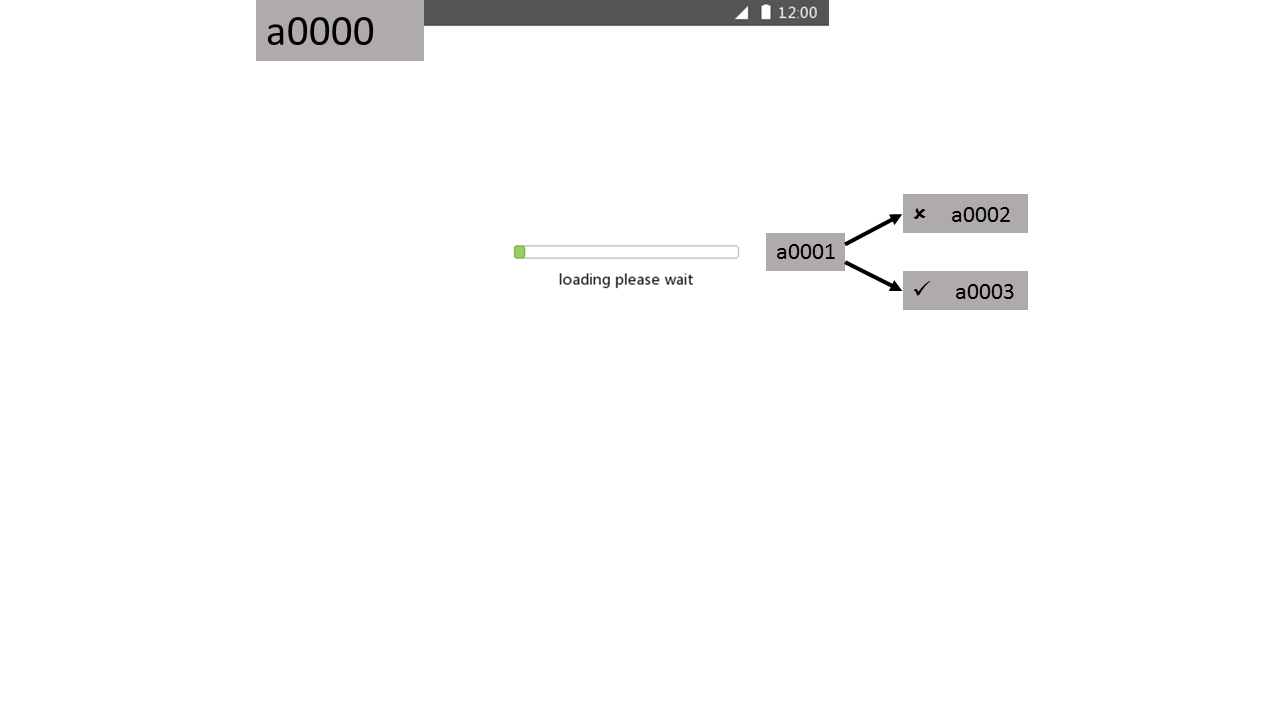
\includegraphics[width=\linewidth,height=\textheight,keepaspectratio]{Dialoge/a0000}
\caption{Starten der Software}
\end{figure}
\FloatBarrier

\subsubsection{Pop-Up a0002}
\begin{figure}[!htbp]
\centering
\noindent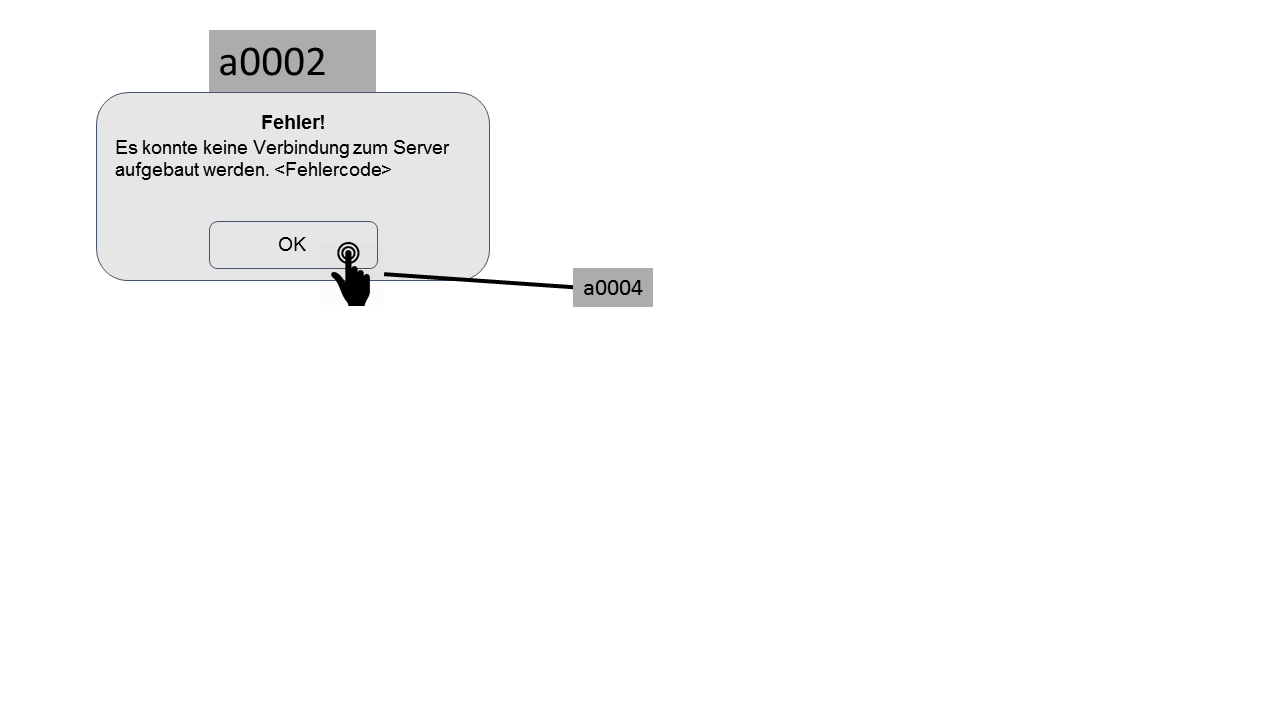
\includegraphics[width=\linewidth,height=\textheight,keepaspectratio]{Dialoge/a0000p}
\caption{Pop-Up a0002}
\end{figure}
\FloatBarrier


\subsubsection{Dialog a0100 – Startseite}
\begin{figure}[!htbp]
\centering
\noindent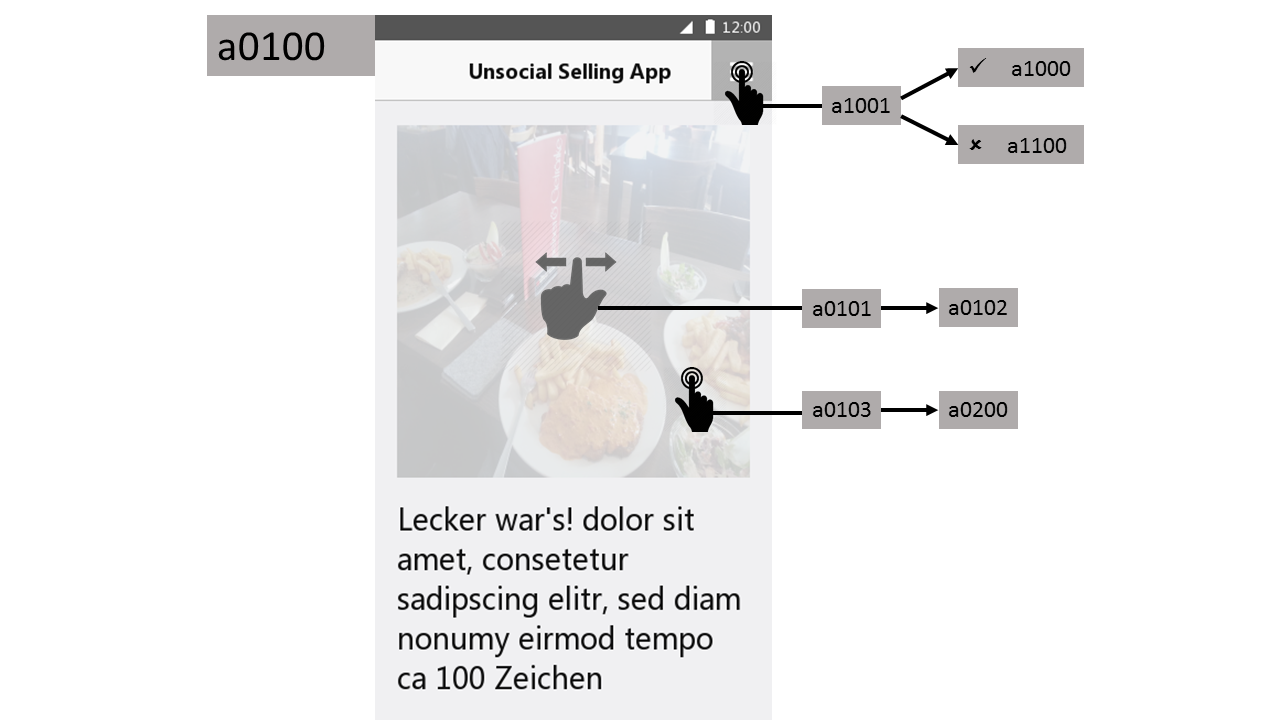
\includegraphics[width=\linewidth,height=\textheight,keepaspectratio]{Dialoge/a0100}
\caption{Startseite}
\end{figure}
\FloatBarrier

\subsubsection{Dialog a0200 – Detailansicht}
\begin{figure}[!htbp]
\centering
\noindent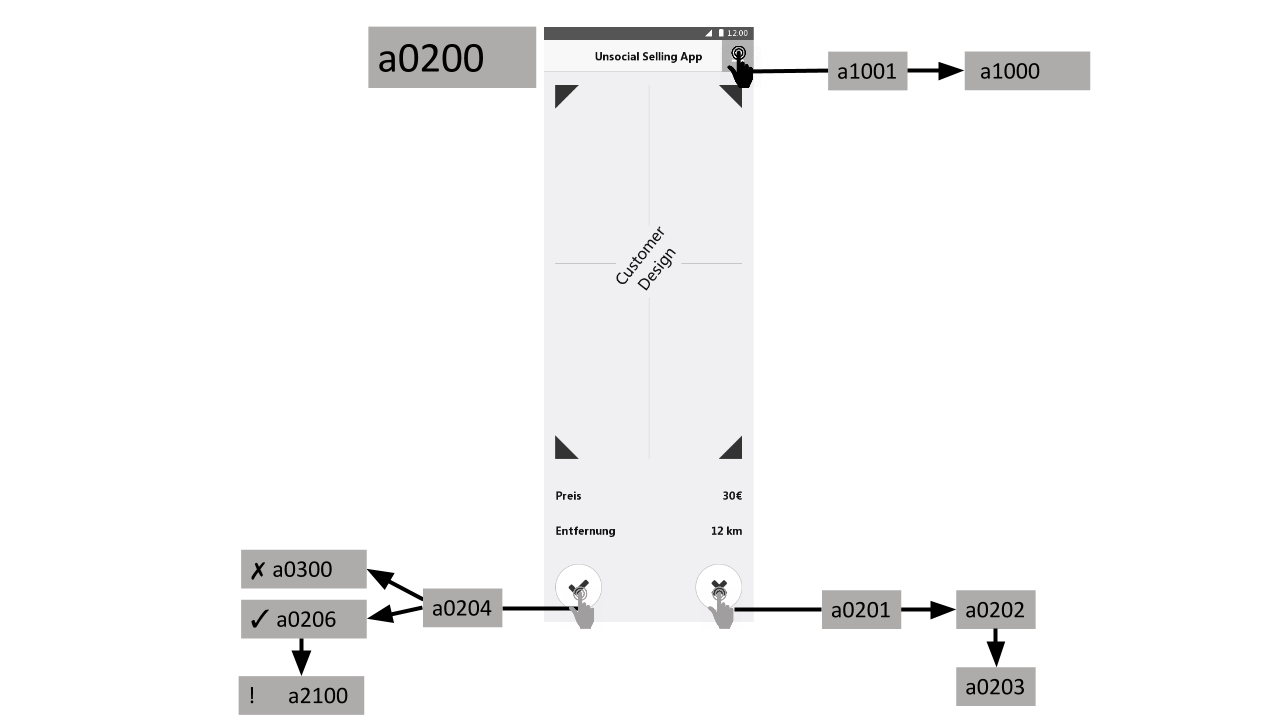
\includegraphics[width=\linewidth,height=\textheight,keepaspectratio]{Dialoge/a0200}
\caption{Detailansicht}
\end{figure}
\FloatBarrier

\subsubsection{Pop-Up a2100 – a2200}
\begin{figure}[!htbp]
\centering
\noindent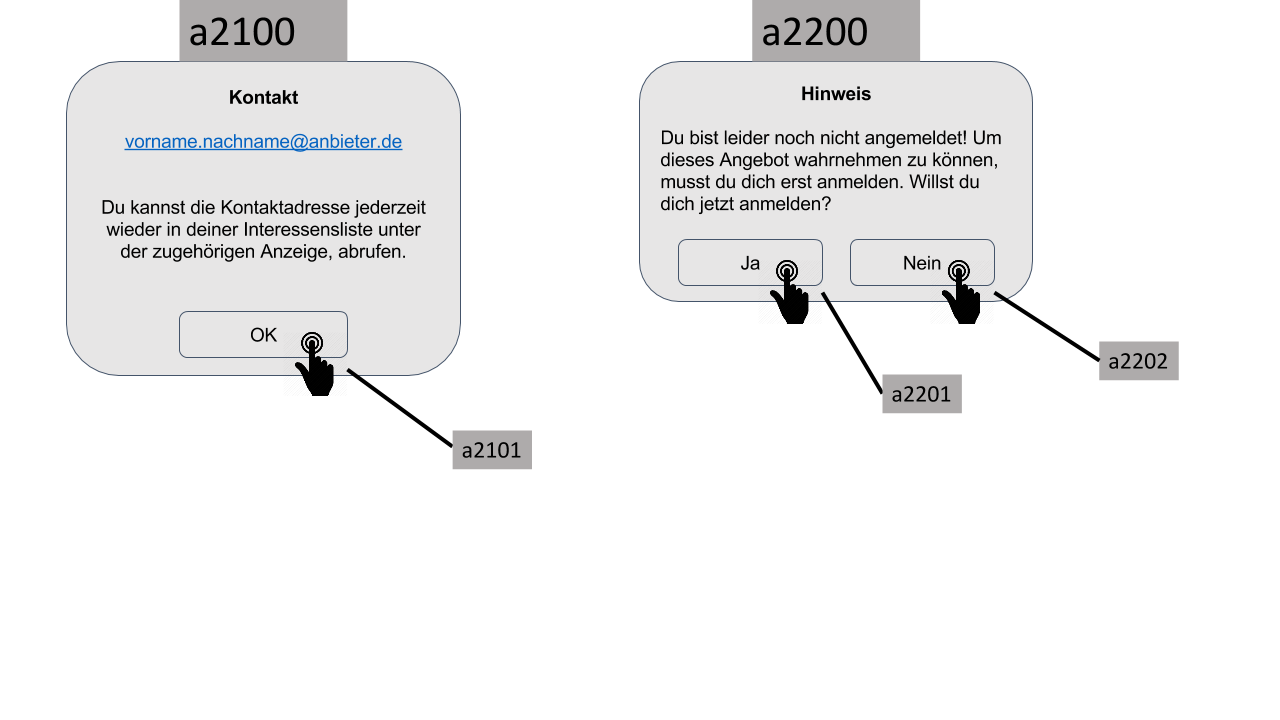
\includegraphics[width=\linewidth,height=\textheight,keepaspectratio]{Dialoge/a0200p}
\caption{Pop-Up a2100 – a2200}
\end{figure}
\FloatBarrier

\subsubsection{Dialog a0300 – Einloggen}
\begin{figure}[!htbp]
\centering
\noindent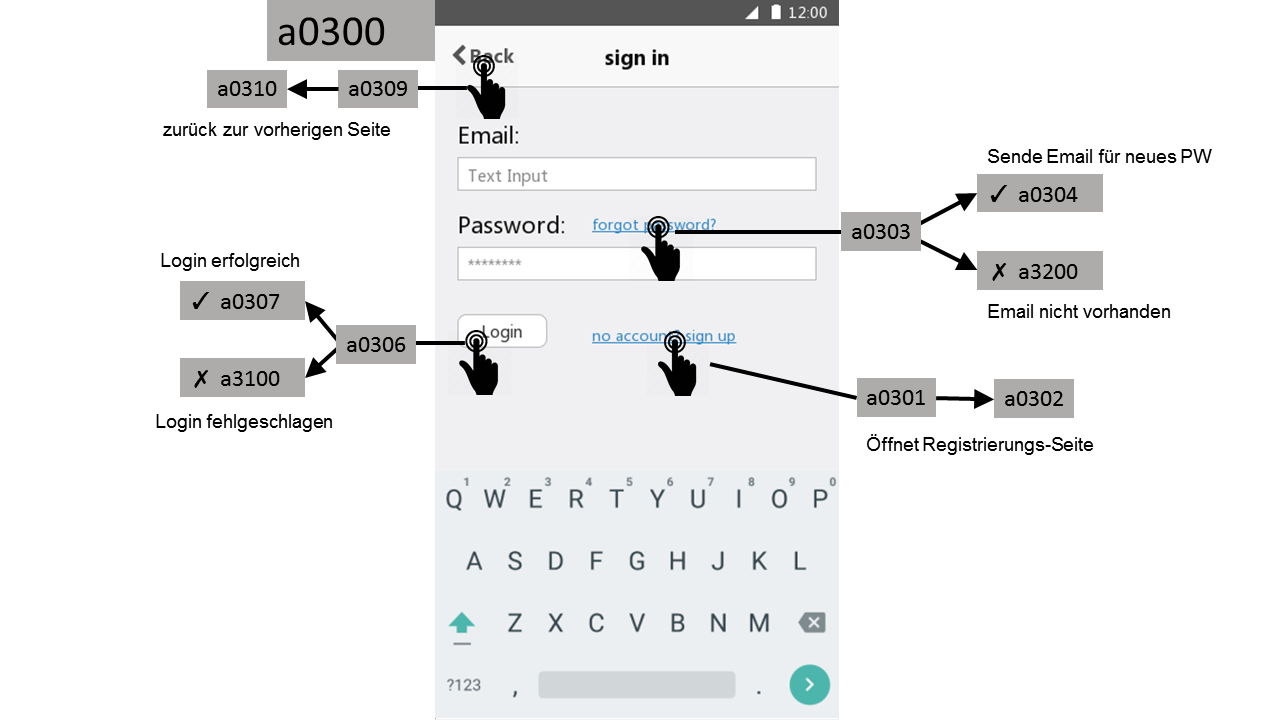
\includegraphics[width=\linewidth,height=\textheight,keepaspectratio]{Dialoge/a0300}
\caption{Einloggen}
\end{figure}
\FloatBarrier

\subsubsection{Pop-Up a3100 – a3200}
\begin{figure}[!htbp]
\centering
\noindent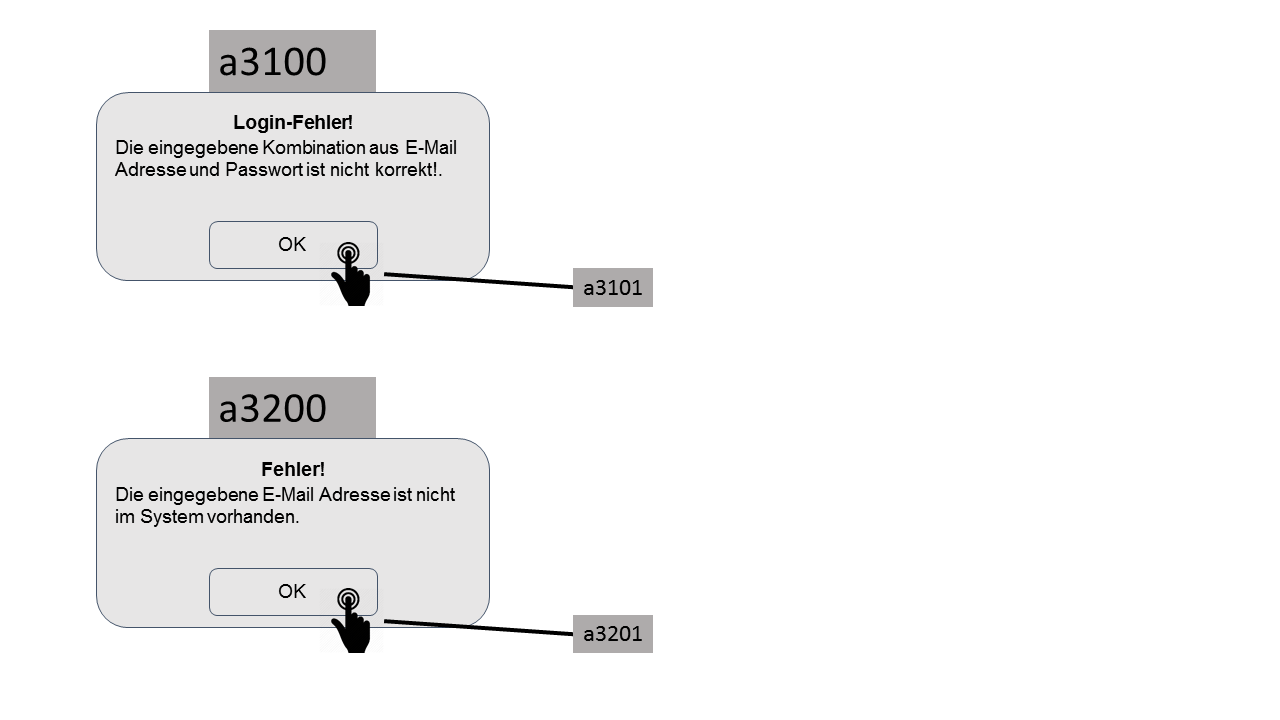
\includegraphics[width=\linewidth,height=\textheight,keepaspectratio]{Dialoge/a0300p}
\caption{Pop-Up a3100 – a3200}
\end{figure}
\FloatBarrier

\subsubsection{Dialog a0400 – Registrieren}
\begin{figure}[!htbp]
\centering
\noindent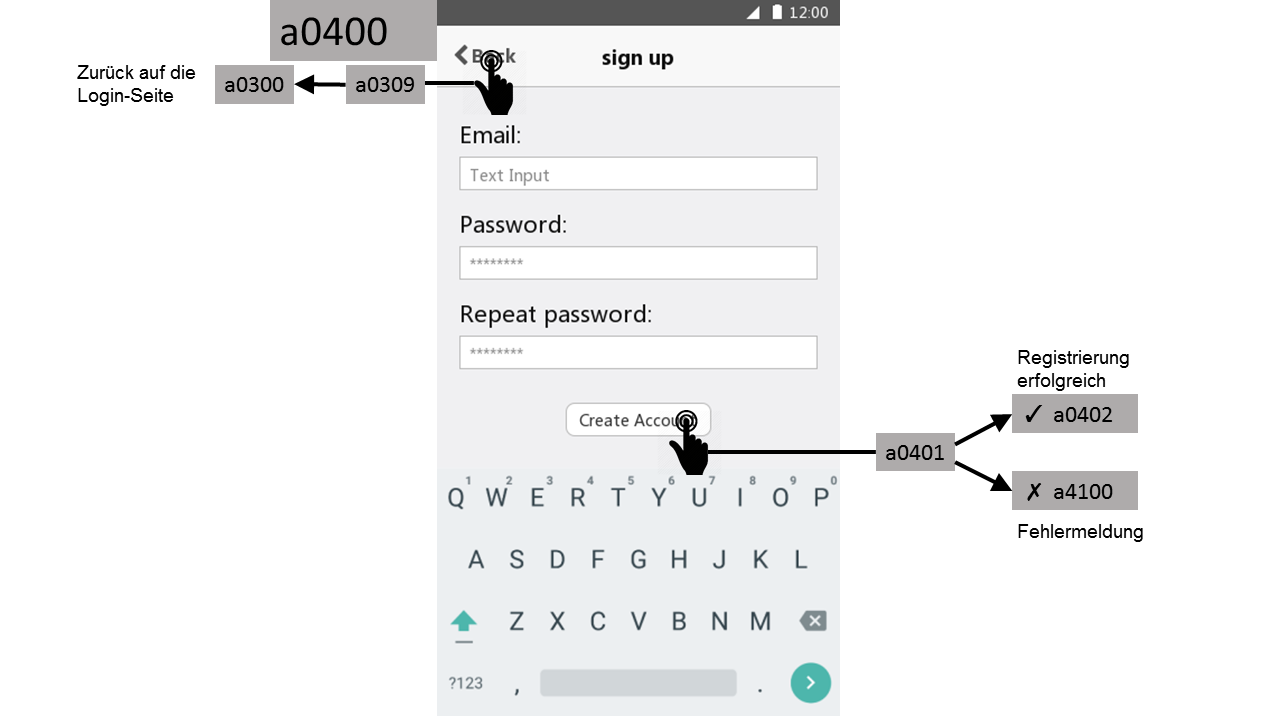
\includegraphics[width=\linewidth,height=\textheight,keepaspectratio]{Dialoge/a0400}
\caption{Registrieren}
\end{figure}
\FloatBarrier

\subsubsection{Pop-Up a4100}
\begin{figure}[!htbp]
\centering
\noindent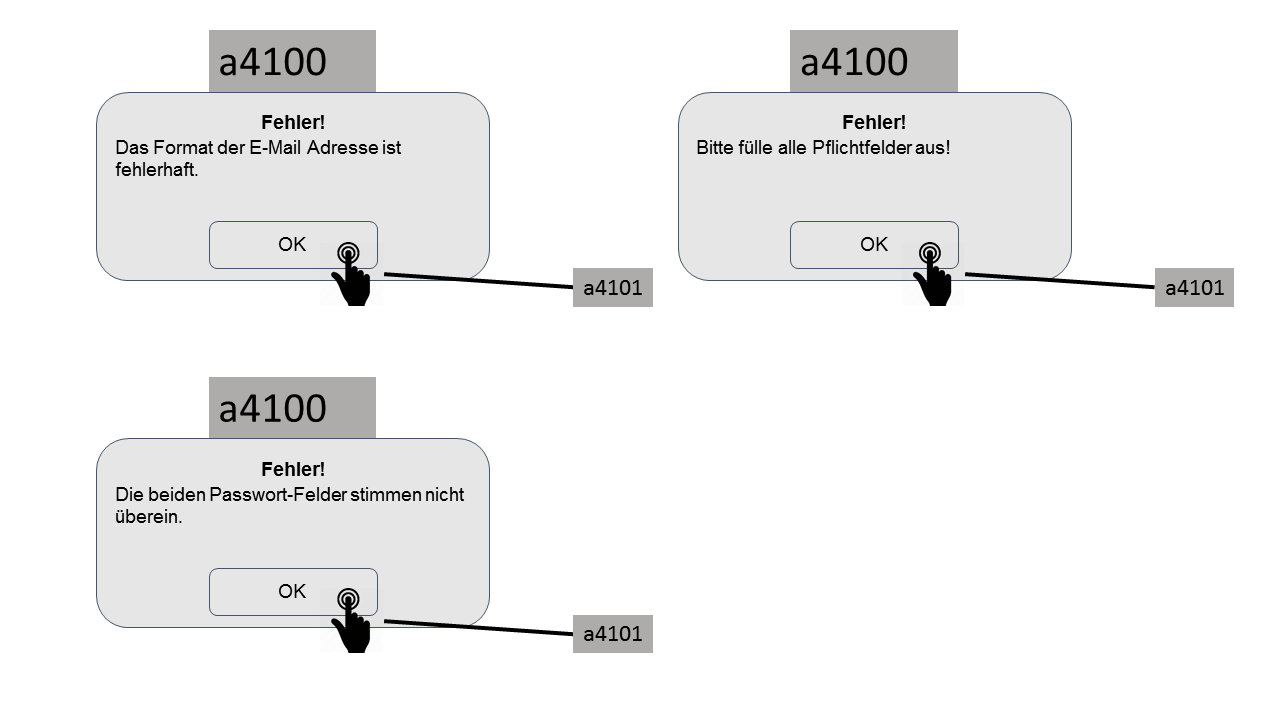
\includegraphics[width=\linewidth,height=\textheight,keepaspectratio]{Dialoge/a0400p}
\caption{Pop-Up a4100}
\end{figure}
\FloatBarrier

\subsubsection{Dialog a0500 – Benutzer Verwaltung}
\begin{figure}[!htbp]
\centering
\noindent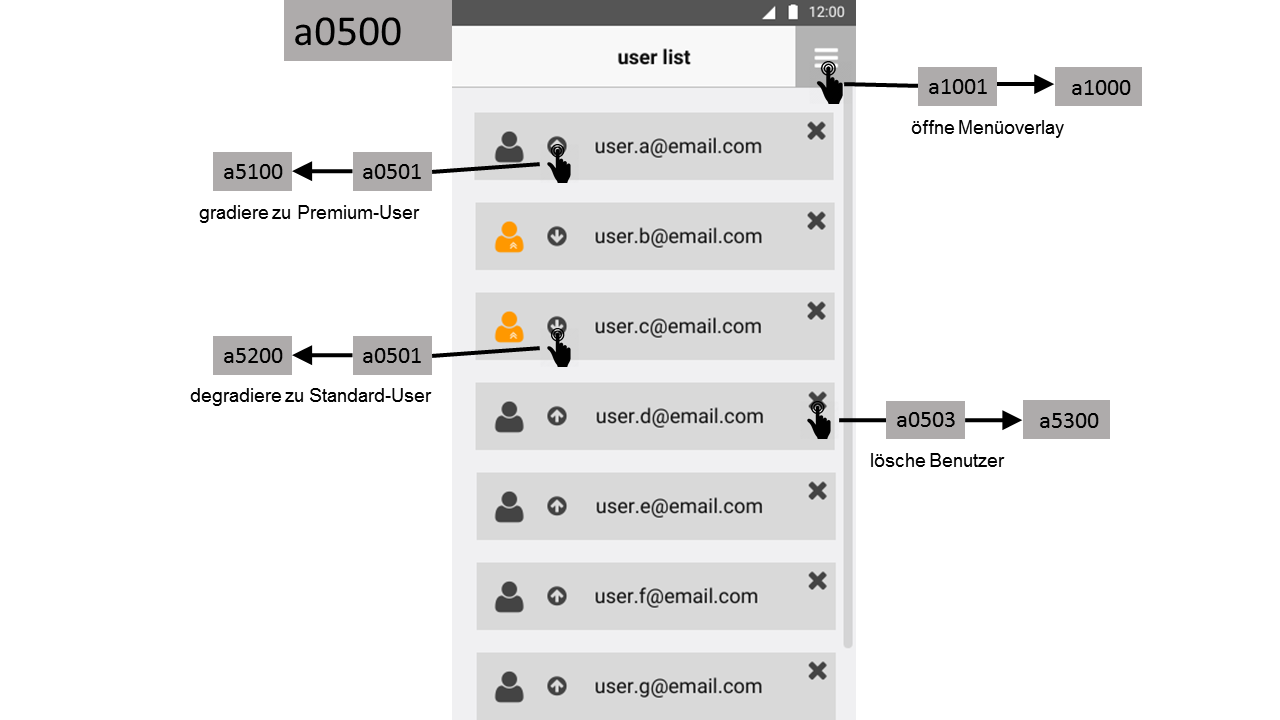
\includegraphics[width=\linewidth,height=\textheight,keepaspectratio]{Dialoge/a0500}
\caption{Benutzer Verwaltung}
\end{figure}
\FloatBarrier

\subsubsection{Pop-Up a5100 – a5300}
\begin{figure}[!htbp]
\centering
\noindent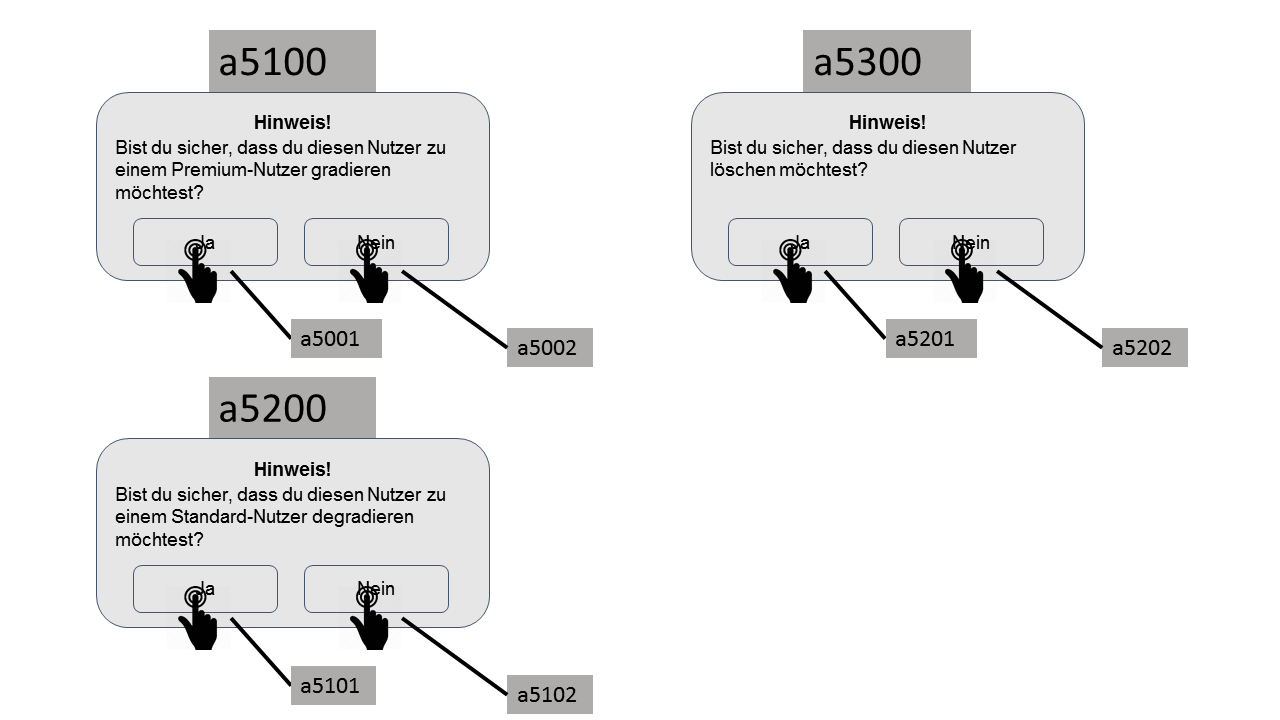
\includegraphics[width=\linewidth,height=\textheight,keepaspectratio]{Dialoge/a0500p}
\caption{Pop-Up a5100 – a5300}
\end{figure}
\FloatBarrier

\subsubsection{Dialog a0600 – Interessen Liste}
\begin{figure}[!htbp]
\centering
\noindent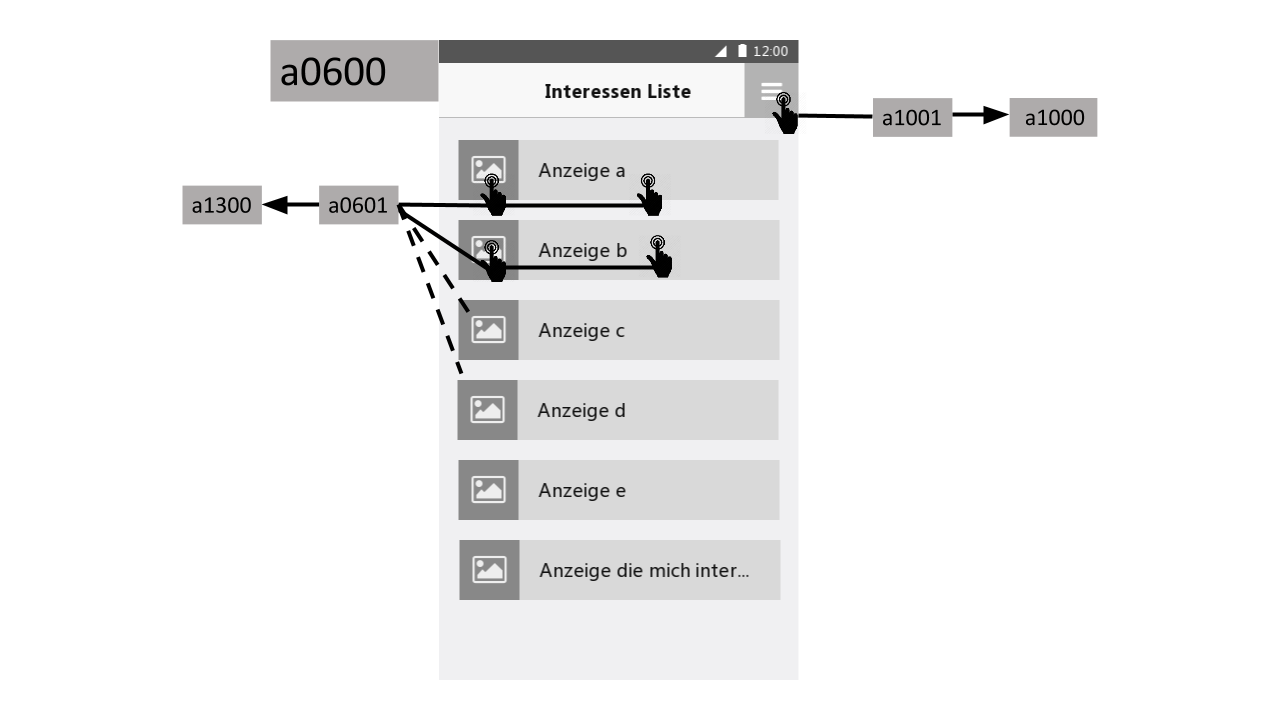
\includegraphics[width=\linewidth,height=\textheight,keepaspectratio]{Dialoge/a0600}
\caption{Interessen Liste}
\end{figure}
\FloatBarrier

\subsubsection{Dialog a0700 – Einstellungen}
\begin{figure}[!htbp]
\centering
\noindent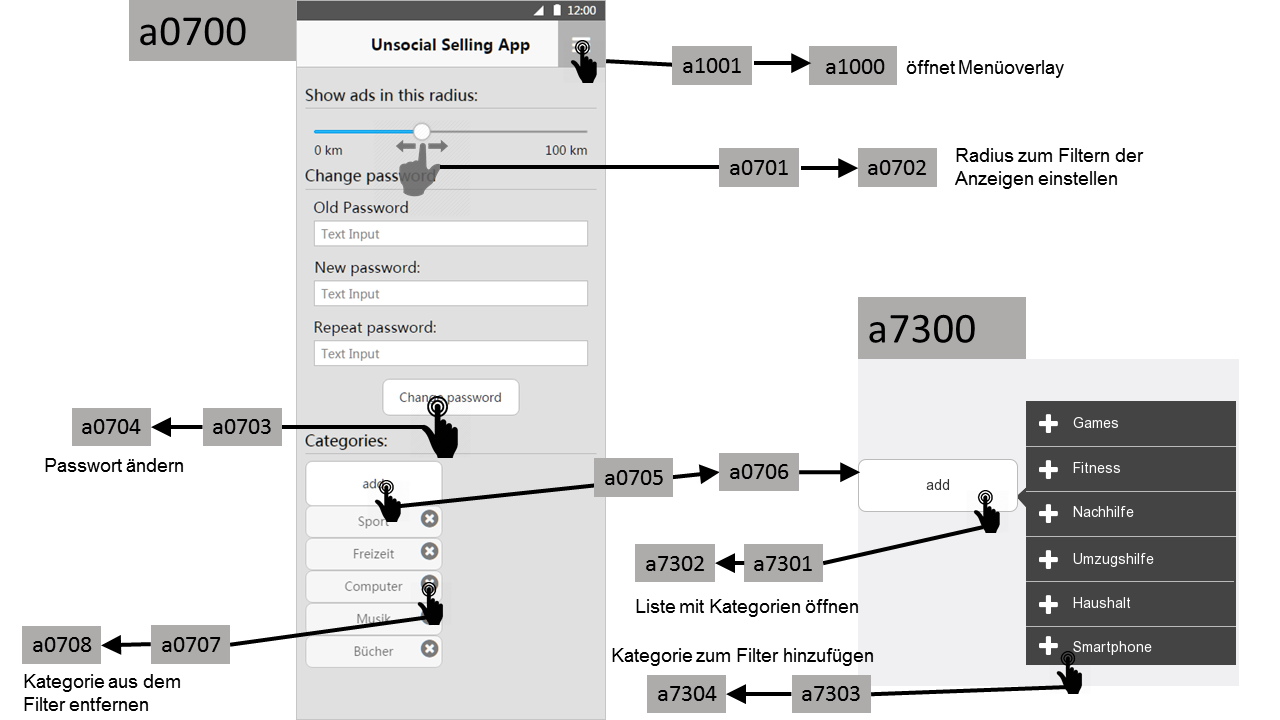
\includegraphics[width=\linewidth,height=\textheight,keepaspectratio]{Dialoge/a0700}
\caption{Einstellungen}
\end{figure}
\FloatBarrier

\subsubsection{Pop-Up a7100 – a7200}
\begin{figure}[!htbp]
\centering
\noindent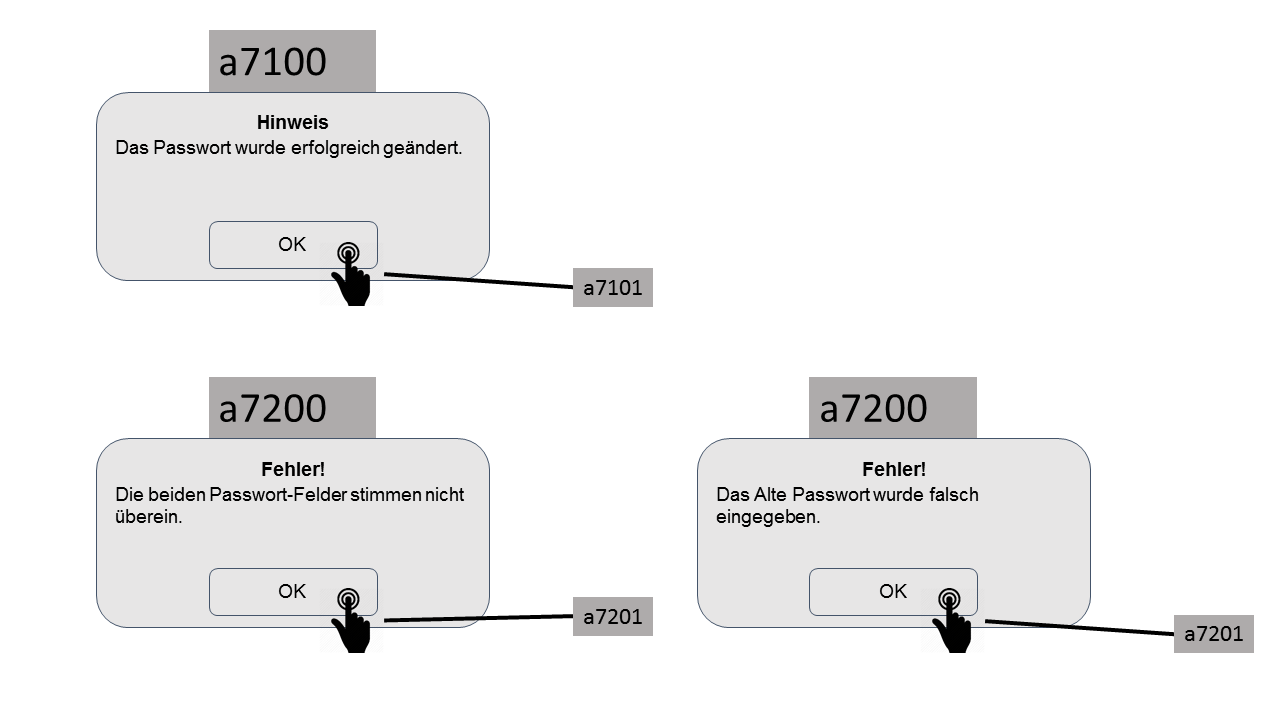
\includegraphics[width=\linewidth,height=\textheight,keepaspectratio]{Dialoge/a0700p}
\caption{Pop-Up a7100 – a7200}
\end{figure}
\FloatBarrier

\subsubsection{Dialog a0800 – eingestellte Anzeigen Liste}
\begin{figure}[!htbp]
\centering
\noindent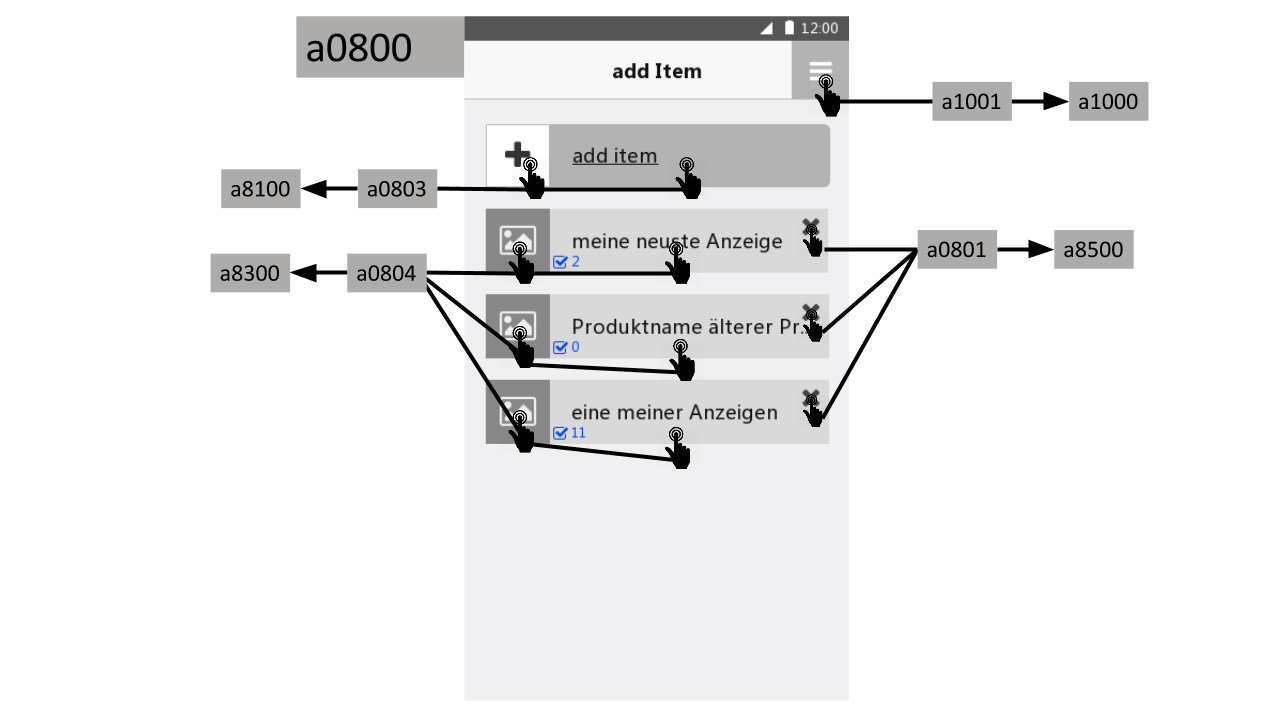
\includegraphics[width=\linewidth,height=\textheight,keepaspectratio]{Dialoge/a0800}
\caption{eingestellte Anzeigen Liste}
\end{figure}
\FloatBarrier

\subsubsection{Pop-Up a8900}
\begin{figure}[!htbp]
\centering
\noindent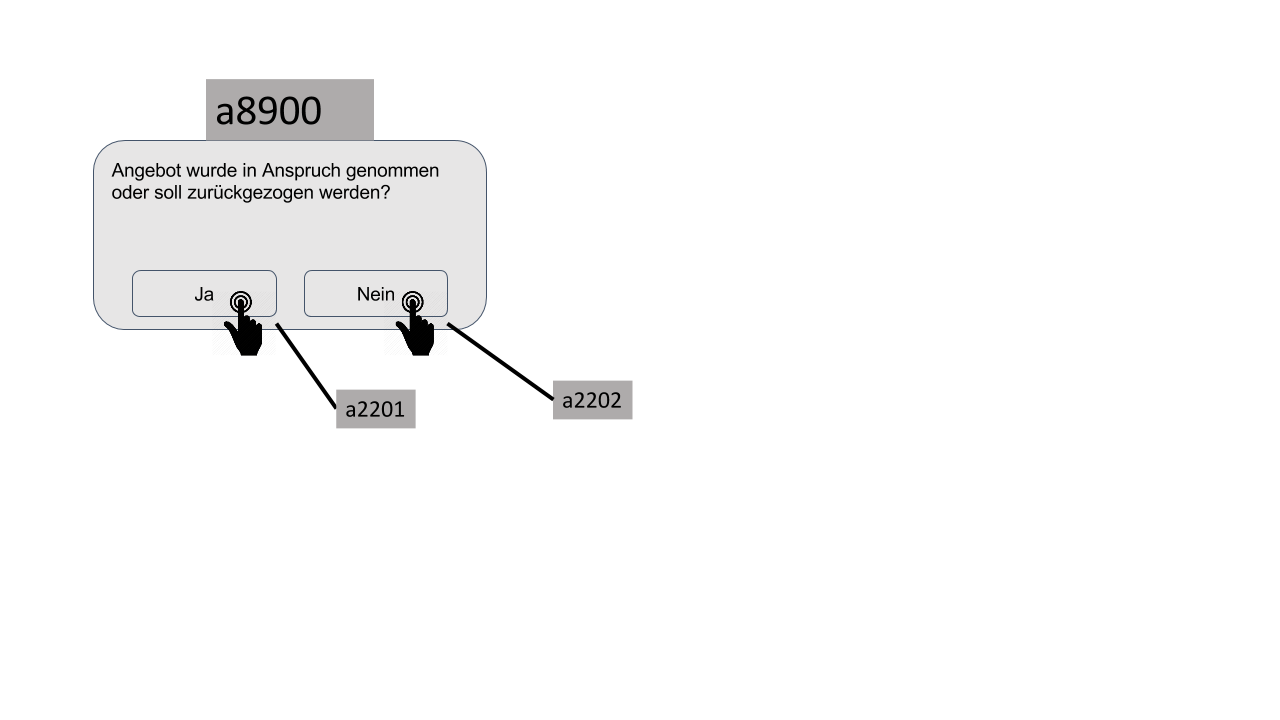
\includegraphics[width=\linewidth,height=\textheight,keepaspectratio]{Dialoge/a8900p}
\caption{Pop-Up a8900}
\end{figure}
\FloatBarrier

\subsubsection{Dialog a8100 – neue Anzeige einstellen }
\begin{figure}[!htbp]
\centering
\noindent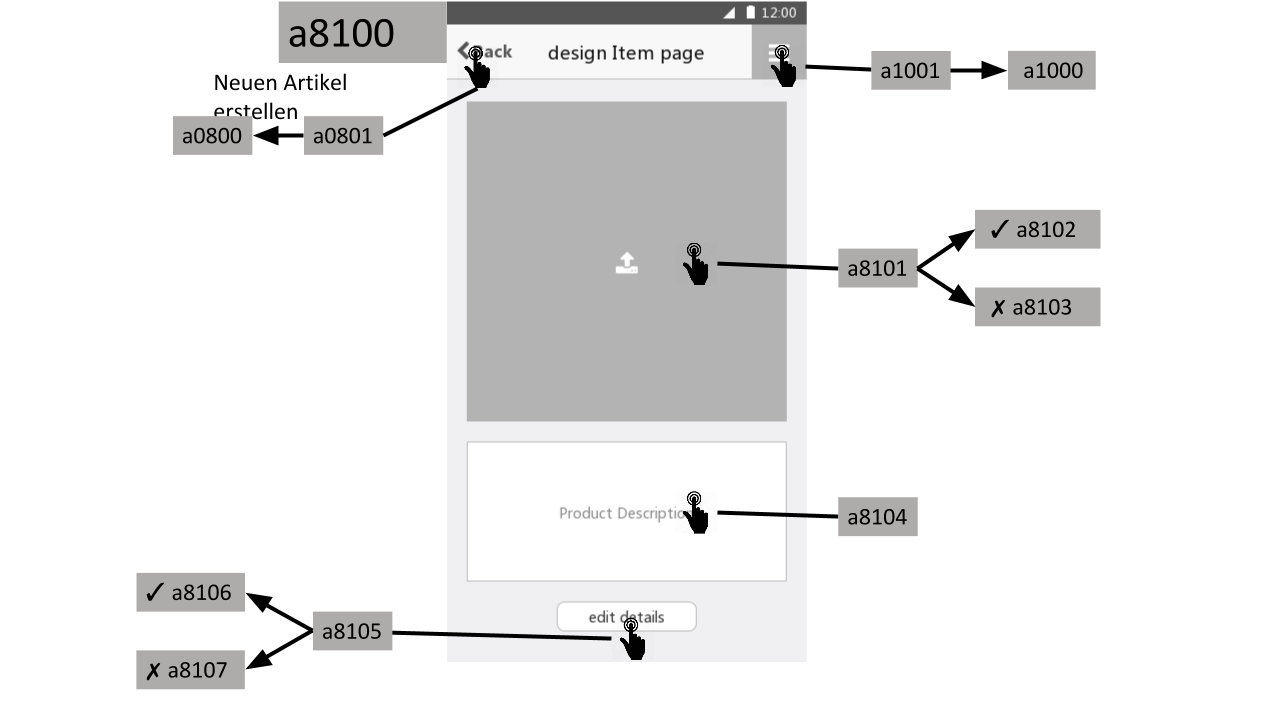
\includegraphics[width=\linewidth,height=\textheight,keepaspectratio]{Dialoge/a8100}
\caption{neue Anzeige einstellen}
\end{figure}
\FloatBarrier

\subsubsection{Pop-Up a8600}
\begin{figure}[!htbp]
\centering
\noindent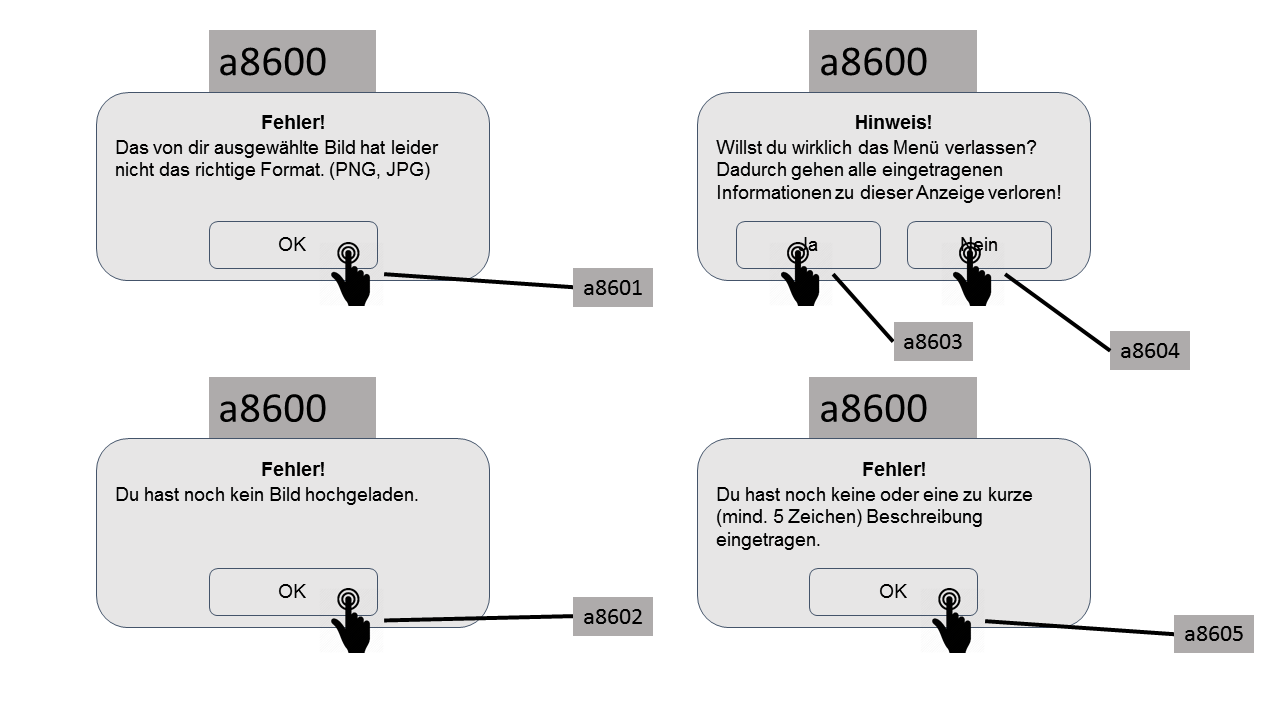
\includegraphics[width=\linewidth,height=\textheight,keepaspectratio]{Dialoge/a8100p}
\caption{Pop-Up a8600}
\end{figure}
\FloatBarrier

\subsubsection{Dialog a8300 – Detailansicht editieren}
\begin{figure}[!htbp]
\centering
\noindent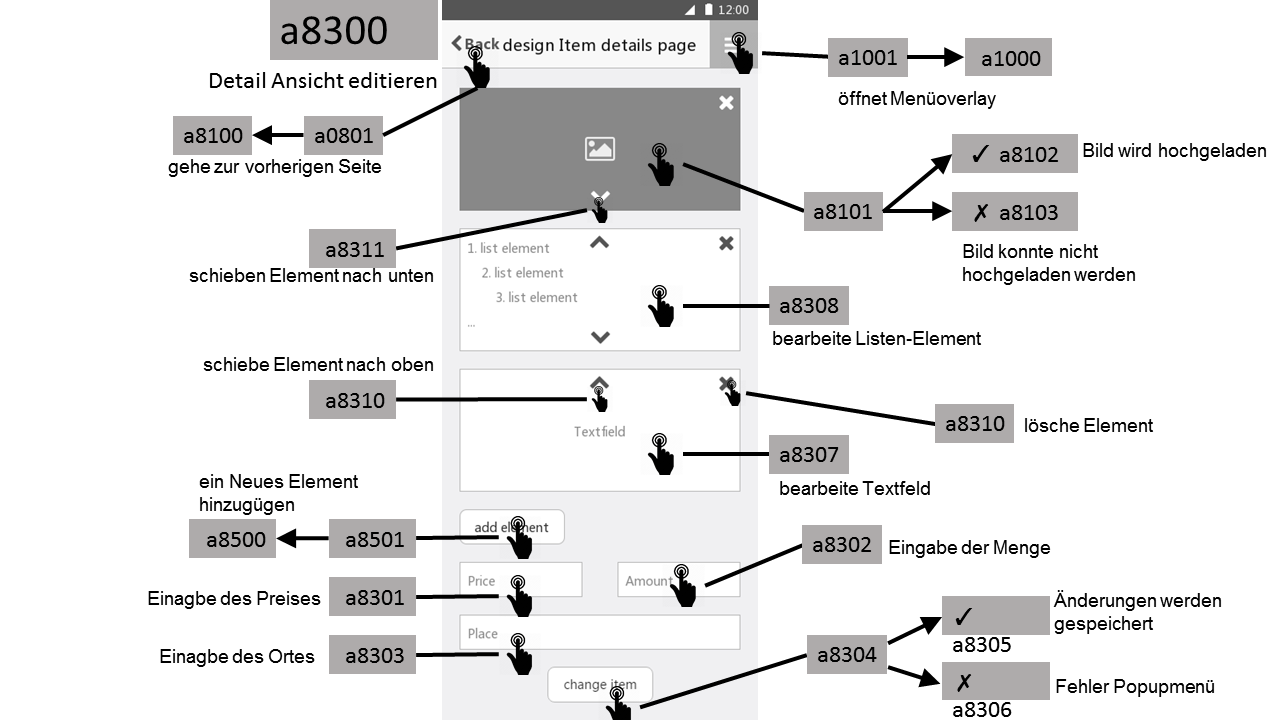
\includegraphics[width=\linewidth,height=\textheight,keepaspectratio]{Dialoge/a8300}
\caption{Detailansicht editieren}
\end{figure}
\FloatBarrier

\subsubsection{Pop-Up a8700}
\begin{figure}[!htbp]
\centering
\noindent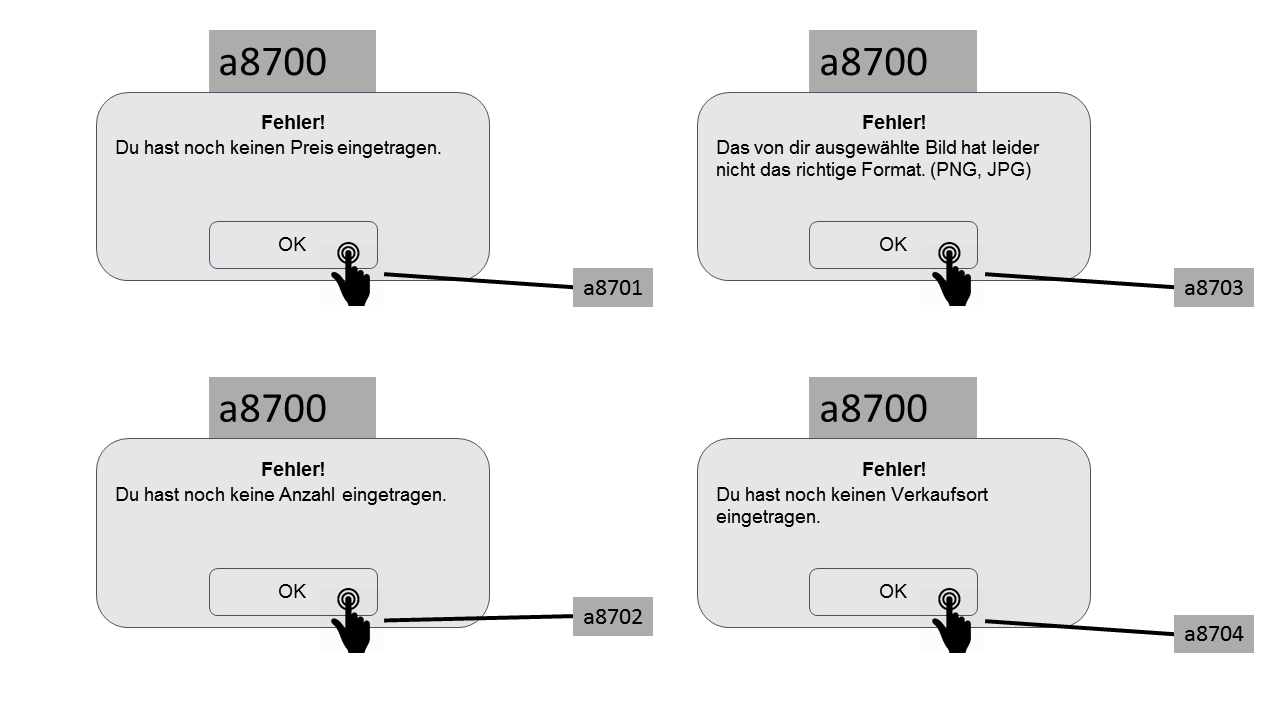
\includegraphics[width=\linewidth,height=\textheight,keepaspectratio]{Dialoge/a8700p}
\caption{Pop-Up a8700}
\end{figure}
\FloatBarrier

\subsubsection{Dialog a8400 – Detailansicht designen}
\begin{figure}[!htbp]
\centering
\noindent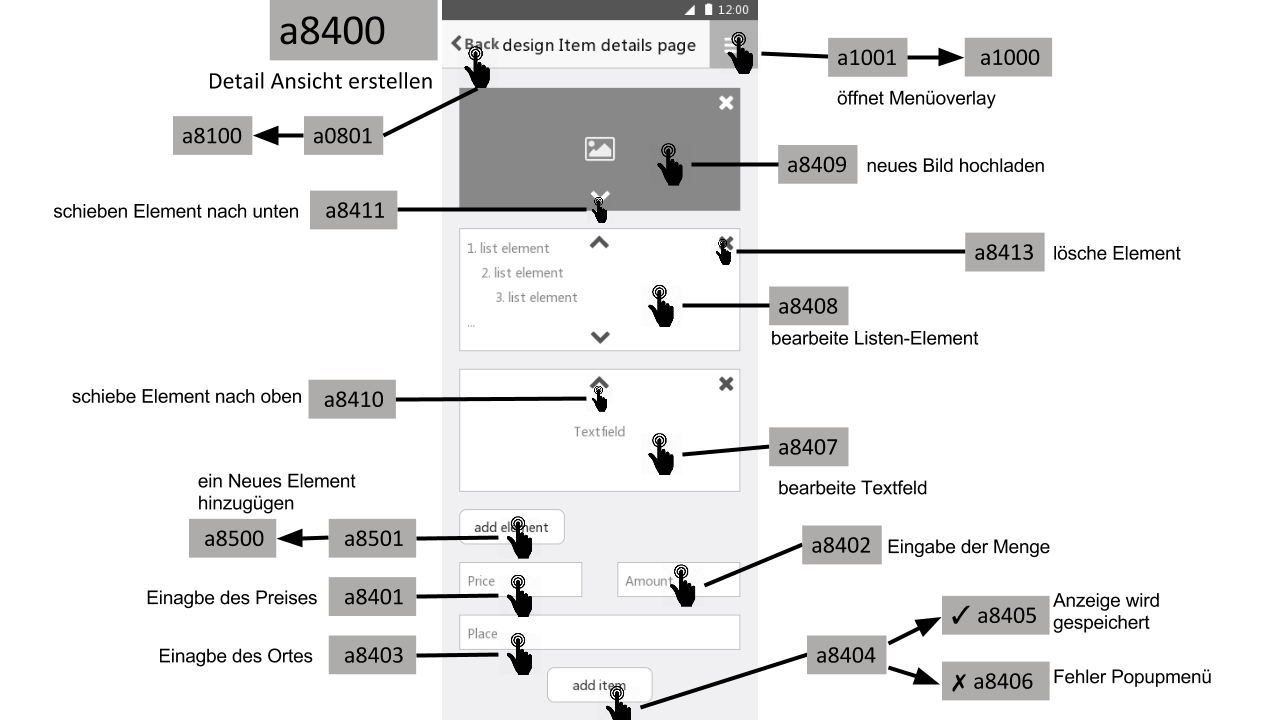
\includegraphics[width=\linewidth,height=\textheight,keepaspectratio]{Dialoge/a8400}
\caption{Detailansicht designen}
\end{figure}
\FloatBarrier

\subsubsection{Pop-Up a8800}
\begin{figure}[!htbp]
\centering
\noindent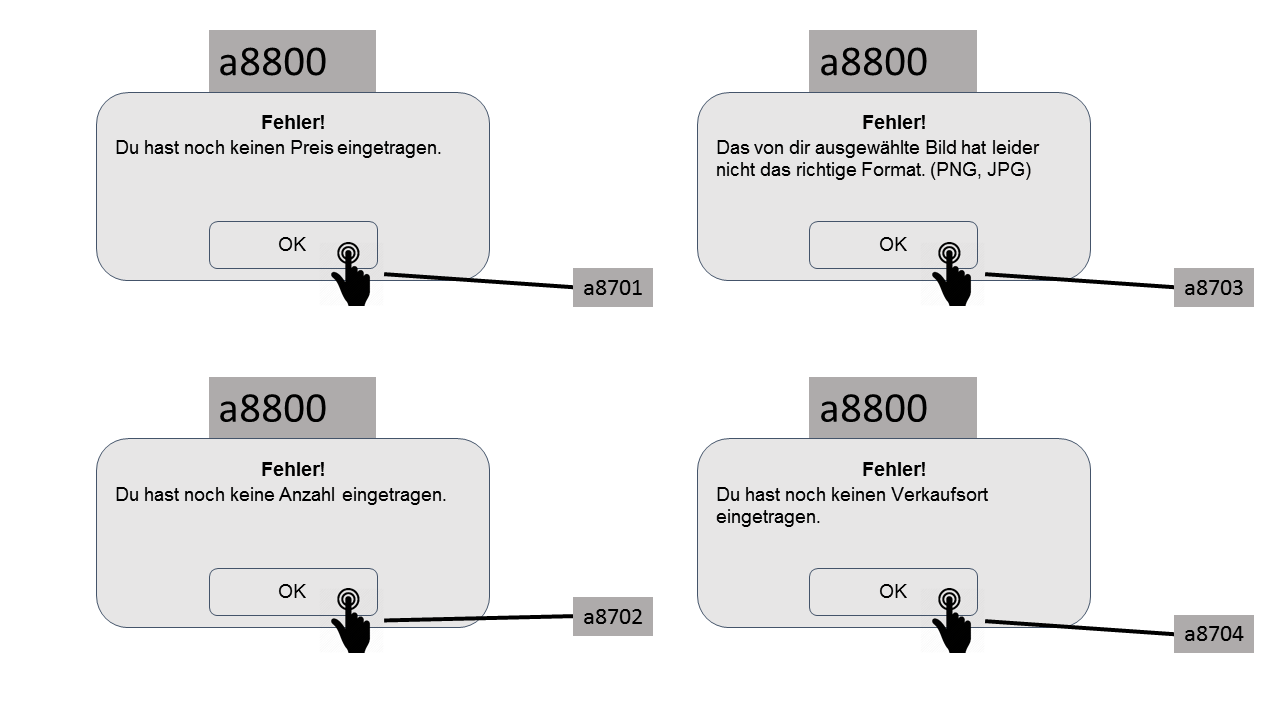
\includegraphics[width=\linewidth,height=\textheight,keepaspectratio]{Dialoge/a8800p}
\caption{Pop-Up a8800}
\end{figure}
\FloatBarrier

\subsubsection{Dialog a8500 – „add Item“ Menü}
\begin{figure}[!htbp]
\centering
\noindent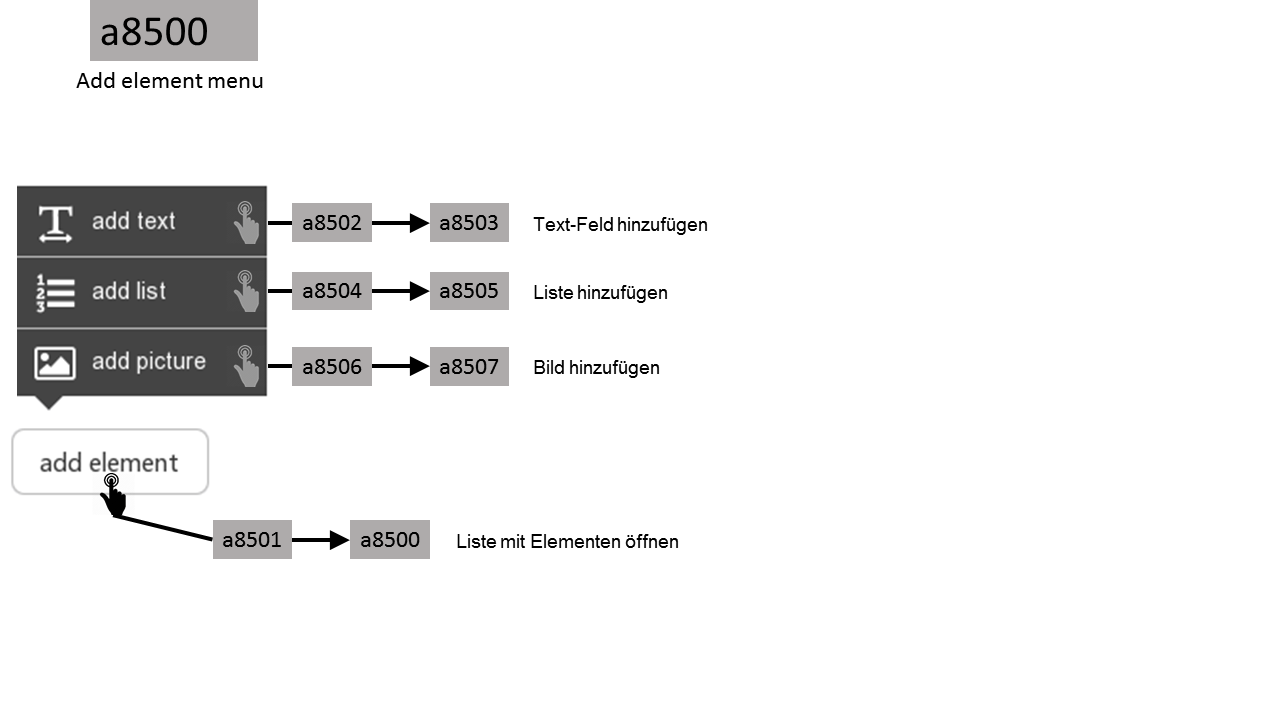
\includegraphics[width=\linewidth,height=\textheight,keepaspectratio]{Dialoge/a8500}
\caption{„add Item“ Menü}
\end{figure}
\FloatBarrier

\subsubsection{Dialog a0900 – Anzeigenverwaltung}
\begin{figure}[!htbp]
\centering
\noindent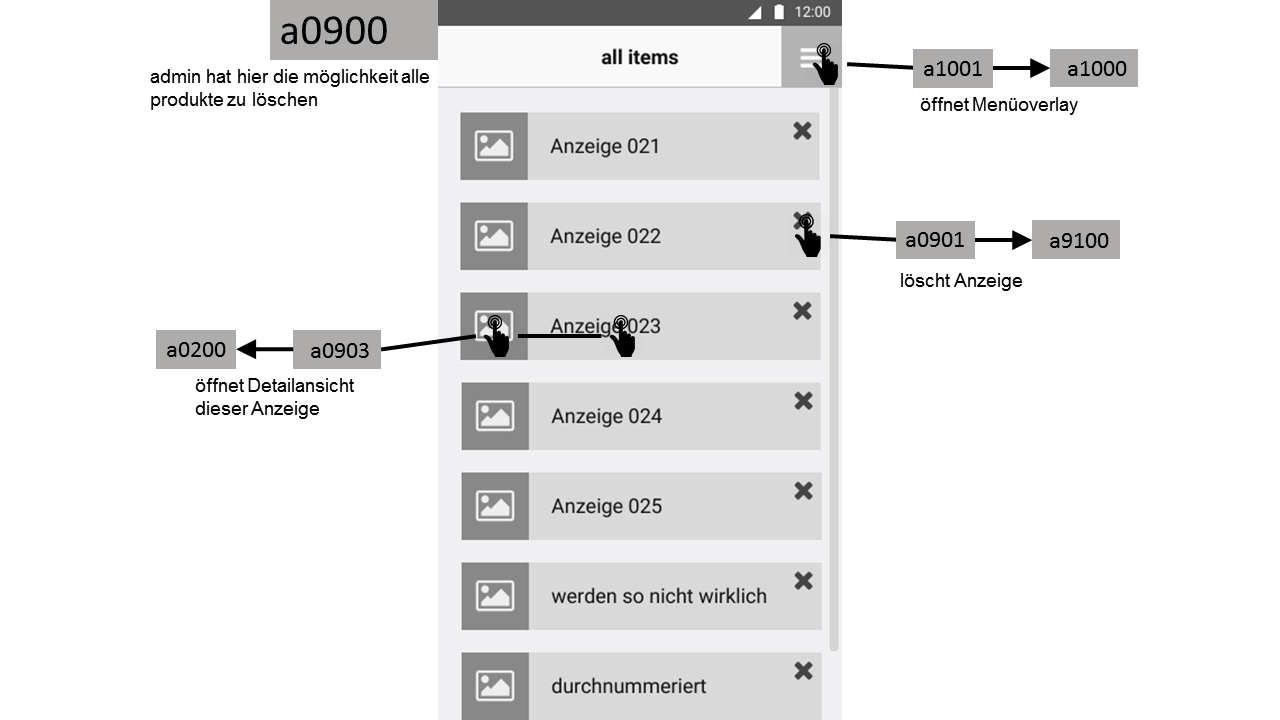
\includegraphics[width=\linewidth,height=\textheight,keepaspectratio]{Dialoge/a0900}
\caption{Anzeigenverwaltung}
\end{figure}
\FloatBarrier

\subsubsection{Pop-Up a9100}
\begin{figure}[!htbp]
\centering
\noindent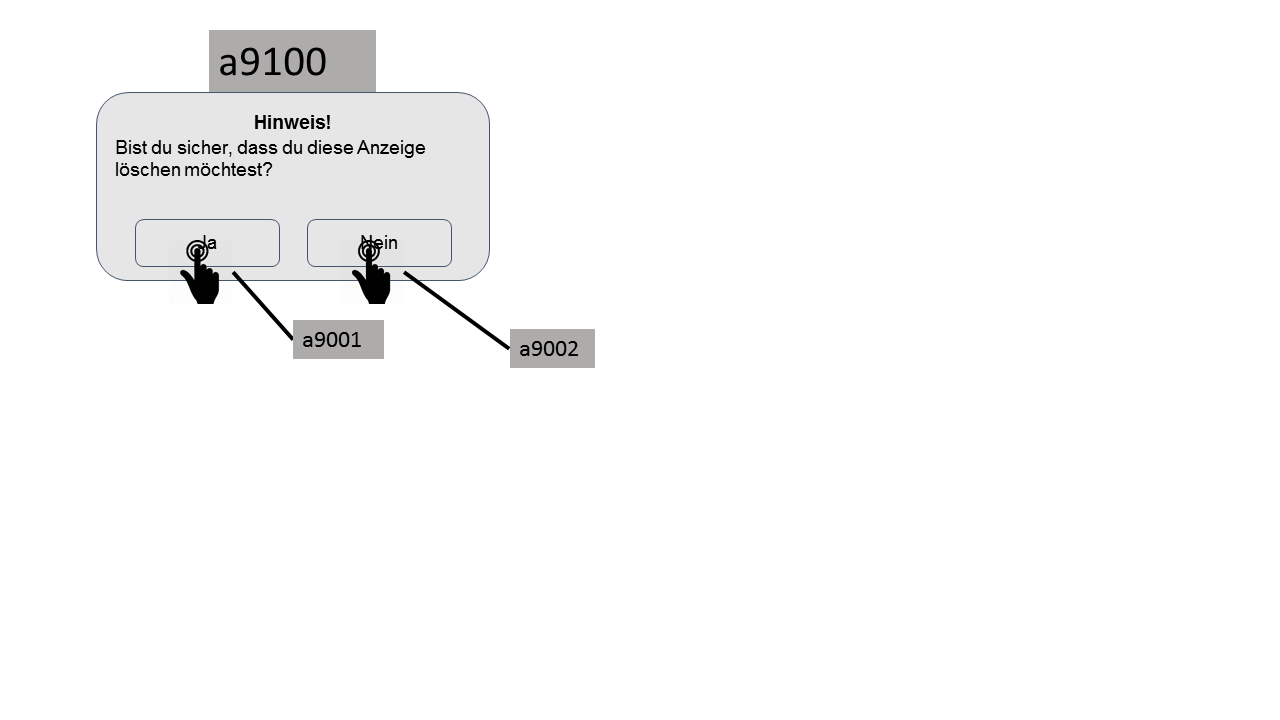
\includegraphics[width=\linewidth,height=\textheight,keepaspectratio]{Dialoge/a9100}
\caption{Pop-Up a9100}
\end{figure}
\FloatBarrier

\subsubsection{Dialog a1000 – Menü}
\begin{figure}[!htbp]
\centering
\noindent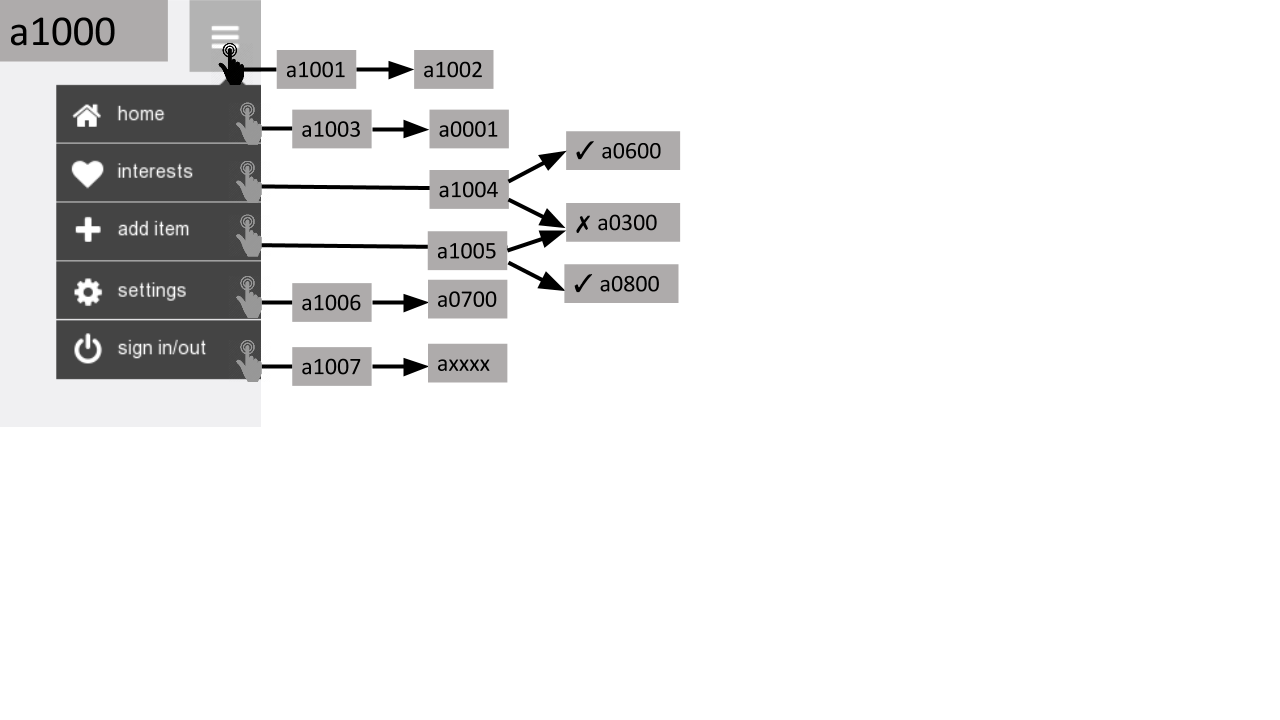
\includegraphics[width=\linewidth,height=\textheight,keepaspectratio]{Dialoge/a1000}
\caption{Menü}
\end{figure}
\FloatBarrier

\subsubsection{Dialog a1100 – Admin Menü}
\begin{figure}[!htbp]
\centering
\noindent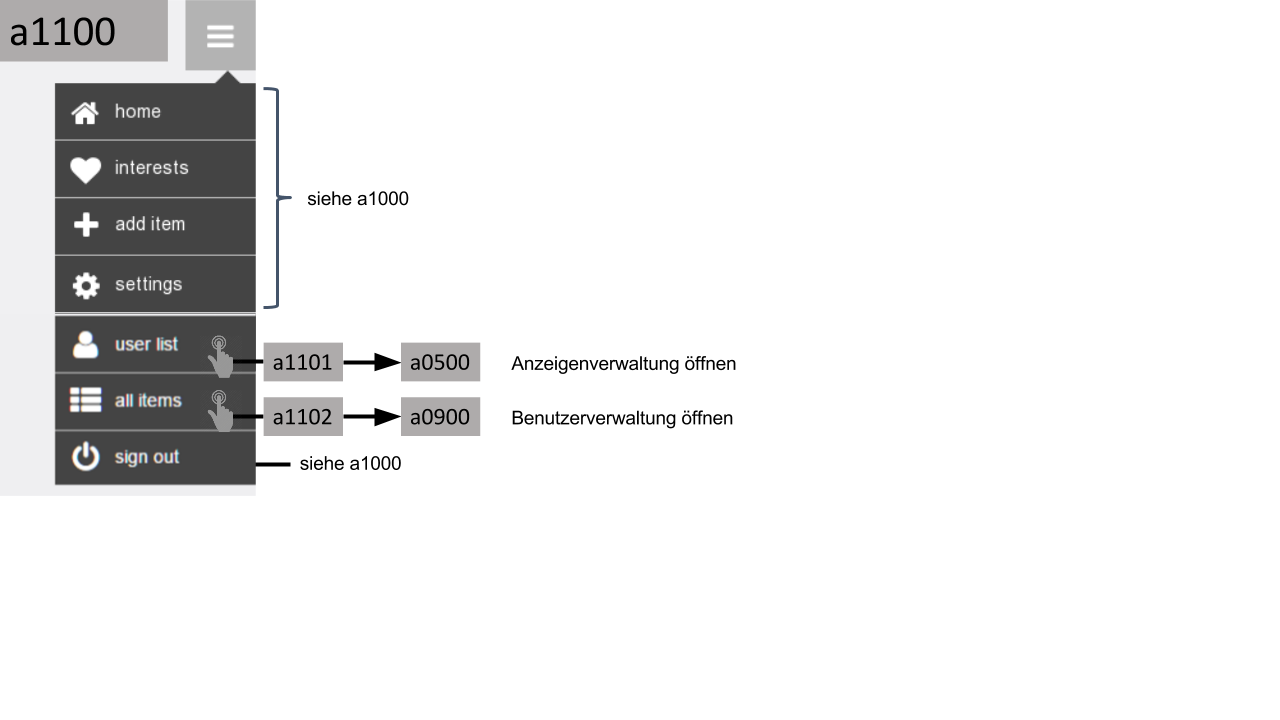
\includegraphics[width=\linewidth,height=\textheight,keepaspectratio]{Dialoge/a1100}
\caption{Admin Menü}
\end{figure}
\FloatBarrier



\section{Produktdaten}
\subsection{Mengengerüst}

\subsubsection*{MENGE\_001 - Benutzeranzahl}
\begin{itemize}
	\item Mit der Software müssen mindestens 300 Personen gleichzeitig arbeiten können. 
	\item Jedem Benutzer muss mindestens 100 MB Speicherplatz zur Verfügung gestellt werden. 
\end{itemize}

\subsubsection*{MENGE\_002 - Anzahl der Vorgänge }
\begin{itemize}
	\item Pro Tag müssen mindestens 25.000 Anzeigen erstellt werden können. 
	\item Pro Tag müssen mindestens 2.500.000 Anzeigen angesehen werden können.
\end{itemize}


\subsection{Vorgaben für Hardware, Software, Schnittstellen}
Die Applikation wird in zwei Teile unterteilt.
Ein Teil ist ein PHP-Server mit einer SQL Datenbank, der Andere, die Client Applikation die auf allen Endgeräten installiert wird.
Der Prototyp, der nachher an den Kunden ausgeliefert wird, muss für Android 5.0 entwickelt werden. 
Da der Source Code auch mit älteren Android Versionen (ab 3.x) und anderen Betriebssystemen (iOS, WinRT und Windows) kompatibel ist, kann der Prototyp mit geringem Aufwand auf andere Plattformen portiert werden.
Optimierung für genaue Modelle ist nicht gefordert.

\subsubsection*{Server}
Auf dem Server werden die Benutzerdaten und Verkaufsdaten in einer Datenbank gespeichert.
Die Benutzerdaten werden nicht an Dritte weitergegeben.
Der Server muss über folgende Ausstattungsmerkmale verfügen:
\begin{itemize}
	\item MySQL 5.5 oder höher bzw. zur DB kompatibel
	\item PHP 5 oder höher bzw. kompatibel
	\item HD mindestens 70 GB
	\item mindestens 4 GB RAM
\end{itemize}

\subsubsection*{Client}
Der Client muss eine ständige Verbindung zum Internet besitzen.
Die Client Applikation muss auf einem Android Smartphone mit Android 5.0 lauffähig sein.

%\textbf{Galaxy Note 2}
%\begin{itemize}
%	\item 5.5 Zoll Display mit einer Auflösung von 720 x 1280 Pixeln
%	\item Quad-core 1.6 GHz Cortex-A9
%	\item Android 4.4 (KitKat)
%	\item 2GB RAM
%\end{itemize} 

%Microsoft Lumia 535
%\begin{itemize}
%	\item 5.0 Zoll Display mit einer Auflösung von 540 x 960 Pixeln
%	\item Quad-core 1.2 GHz Cortex-A7
%	\item Windows Phone Version 8.1
%	\item 1GB RAM
%\end{itemize} 




\section{Produktleistungen}
\hypertarget{s07}{\subsection{Performance}}
Der Server muss innerhalb von 5 Sekunden nach Erhalt einer Anfrage der Clients auf diese antworten.
Dem Benutzer muss bei Wartezeiten eine Warteanzeige abhängig des jeweiligen Betriebssystems angezeigt werden. 
Die RTT "`Round Trip Time"' zwischen Client Anfrage und Server Antwort darf 10 Sekunden nicht überschreiten.
Ist die RTT größer als 10 Sekunden, gilt die Anfrage als fehlgeschlagen.
In diesem Fall muss dem Benutzer eine ausführliche Fehlermeldung angezeigt werden, mit der Möglichkeit, die Anfrage zu wiederholen. 




\section{Qualitätsanforderungen}
Die erstellte Software ist ein Prototyp für ein Konzept und nicht für den realen Einsatz gedacht.
%Weder wird auf Datenschutzbestimmung Rücksicht genommen noch auf etwaige Schäden an Hard- und Software.
%Für diese Haftet alleine der Benutzer.
Alle Funktionen des Prototypen sind auf andere Plattformen, sofern technisch möglich, verfügbar.


\subsection{Bedienbarkeit, Zuverlässigkeit, Effizienz}
Jeder Benutzer muss sich mit seiner E-Mail-Adresse und seinem Passwort beim Server authentifizieren. 
Im lokalen Cache der Client Applikation wird gespeichert, wenn sich ein Benutzer erfolgreich eingeloggt hat. 
Bei erneutem Starten der Applikation wird dieser Benutzer automatisch wieder eingeloggt. 

Der Benutzer darf nur seine eigenen Daten und Aktionen verändern.

%Der Client muss unter Android und sollte auf iOS und WinRT laufen.


\subsubsection{Anforderung an die Zuverlässigkeit}
Die Konsistenz der Datenbank muss jederzeit gewährleistet werden.
Sollte es einen Fehler im System geben, wird die Datenbank auf den letzten noch konsistenten Zustand zurückgesetzt.

Passwörter der Benutzer müssen als MD5-Hash abgespeichert werden.


\subsubsection{Anforderungen an die Benutzbarkeit und des Speicherplatzes}
Die Applikation sollte 50MB Speicherplatz auf dem Smartphone nicht überschreiten. 
Davon werden etwa 10MB für lokale Cache Daten verwendet.
Der Benutzer selbst ist dafür verantwortlich, dass der Applikation genug Speicherplatz zur Verfügung steht. 


\subsubsection{Anforderungen an die Effizienz}
Das Applikation muss innerhalb von 5 Sekunden starten.
Danach muss innerhalb von 10 Sekunden eine Verbindung zum Server aufgebaut sein oder eine Fehlermeldung angezeigt werden.
Siehe \hyperlink{s07}{Kapitel 7.1}.


\subsubsection{Anforderungen an die Änderbarkeit}
Weder Änderungen an einzelnen Komponenten der Anwendung noch am Server oder der Datenbank sollten die gesamte Software beeinträchtigen.
Auch die Integrität sollte nicht beeinträchtigt sein.


\subsubsection{Anforderungen an den Schutz der Systemumgebung und an den Schutz des Systems}
Jeder Benutzer des Systems muss sich bei der Anmeldung am Server über die Applikation mittels E-Mail und Passwort authentifizieren.
Der Server erstellt für die weiteren Sitzungen eine eindeutige ID, mit der sich die Client Applikation im weiteren Verlauf der Benutzung bei jeder Aktion am Server autorisiert.
Die ID ist solange gültig, bis der Benutzer sich abmeldet oder der Server die Sitzung beendet.
Der Server hebt die Gültigkeit einer ID auf, wenn der Benutzer 12 Stunden nicht mehr aktiv war.
Der Benutzer darf nur seine eigenen Daten und Anzeigen verändern, was mittels Autorisierung sichergestellt wird.
Der System-Administrator hat Zugriff auf alle Daten dieser Datenbank, da er die Datenbank verwaltet. 

Die Software soll unter Einhaltung des BSI-Grundschutzes erstellt werden. 



\end{document}
